%%%%%%%%%%%%%%%%%%%%%%%%%%%%%%%%%%%%%%%%%
% OIST Doctoral Thesis - Final bound version
% LaTeX Template
% Version 0.2 (2016/04/06)
%
% This version is the final binding version which will be published.
%
%%%%%%%%%%%%%%%%%%%%%%%%%%%%%%%%%%%%%%%%%

%----------------------------------------------------------------------------------------
%	PACKAGES AND OTHER DOCUMENT CONFIGURATIONS
%----------------------------------------------------------------------------------------

\documentclass[12pt, twoside]{book} % 12 pt font, two-sided book style
\usepackage[a4paper, includehead, headheight=0.6cm, inner=3cm ,outer=2.5cm, top=2.5 cm, bottom=2.5cm]{geometry}  % Changing size of document
\usepackage[english]{babel} % The document is in English
\usepackage[utf8]{inputenc} % UTF8 encoding
\usepackage[T1]{fontenc} % Font encoding

\usepackage{graphicx} % For including images
\graphicspath{{./Images/}} % Specifies the directory where pictures are stored

\usepackage{longtable} % tables that can span several pages
\usepackage[bf]{caption} % caption: FIG in bold
\usepackage{fancyhdr} % For the headers

\newcommand{\numberedchapter}{ % Preparation for numbered chapters
	\cleardoublepage % To make sure the previous headers are passed
	\fancyhead[RE]{{\bfseries \leftmark}}% Headers for left pages
	\fancyhead[LO]{{\bfseries \rightmark}}}% Headers for right pages
\newcommand{\unnumberedchapter}[1]{ % Preparation for unnumbered chapters
	\cleardoublepage % To make sure the previous headers are passed
	\addcontentsline{toc}{chapter}{#1} % Also adds the chapter name to the Contents
	\fancyhead[RE]{{\bfseries #1}} % Headers for left pages
	\fancyhead[LO]{}}%Headers for right pages

\usepackage{emptypage} % No headers on an empty page

\usepackage{eso-pic} % For the background picture on the title page
\newcommand\BackgroundPic{%
\put(-250,-160){%
\parbox[b][\paperheight]{\paperwidth}{%
\vfill
\centering
\includegraphics[width=\paperwidth]{symbol.jpg}%
\vfill
}}}

% plug-in packages
\usepackage[utf8]{inputenc}
\usepackage[maxcitenames=1]{biblatex}
\usepackage{amsmath}
\usepackage{amssymb}
\usepackage{amsthm}
\usepackage{tcolorbox}
\usepackage{graphicx}
\usepackage{algorithm}
\usepackage{algorithmic}
\usepackage{subfig}
\usepackage{hyperref}
\usepackage{cleveref}
\usepackage{thmtools}
\usepackage{thm-restate}
\usepackage{enumerate}

%------------------------------------------------------------------

% theorem env setting
\theoremstyle{plain}
\newtheorem{lemma}{Lemma}
\newtheorem{theo}{Theorem}
\newtheorem{prop}{Proposition}
\newtheorem{defi}{Definition}
\newtheorem{coro}{Corollary}
\newtheorem{policy}{Policy}
\newtheorem{ass}{Assumption}

%------------------------------------------------------------------

% command definition
% sum of expectation of sup-optimal draws of each arm
\newcommand{\sd}{\mathbb{E}[\Psi_N]}
% the percent of optimal arm is drawn
\newcommand{\opt}{O_N}
\newcommand{\de}{\mathrm{d}}
\DeclareMathOperator*{\argmax}{argmax}
\DeclareMathOperator*{\argmin}{argmin}
%\DeclareMathOperator*{\min}{min}

\newcommand{\ourtitle}{Median-based Bandits for Unbounded Rewards}
\newcommand{\ourpolicy}{M-UCB}

\newcommand{\cheng}[1]{\textcolor{magenta}{\bf Cheng: #1}}

\newenvironment{proof-sketch}{\noindent{\textit{Sketch of Proof.}}\hspace*{1em}}{\qed\bigskip}


%----------------------------------------------------------------------------------------
%	ADD YOUR CUSTOM VALUES, COMMANDS AND PACKAGES
%----------------------------------------------------------------------------------------

% Open Preamble/mydefinitions.tex and enter some values (name, thesis title...) 
% and include your own custom LaTeX functions and packages

%----------------------------------------------------------------------------------------
%	VALUES FOR THE THESIS
%----------------------------------------------------------------------------------------

\newcommand{\name}{Mengyan Zhang} % Author name
\newcommand{\thesistitle}{Bandits} % Title of the thesis
\newcommand{\submissiondate}{October, 2019} % Submission date "Month, year"
\newcommand{\advisor}{Cheng Soon Ong, Lexing Xie, Eduardo Eyras} % Supervisor name
\newcommand{\coadvisor}{Someone Someone} % Co-Supervisor name, comment this line if there is none


%----------------------------------------------------------------------------------------
%	BIBLIOGRAPHY STYLE (pick the style you want)
%----------------------------------------------------------------------------------------

%\usepackage[square, numbers, sort&compress]{natbib} % for bibliography - Square brackets, citing references with numbers, citations sorted by appearance in the text and compressed (as in [4-7])
%\usepackage[longnamesfirst,round]{natbib} % Natural Sciences bibliography

%\bibliographystyle{Preamble/physics_bibstyle} % You may use a different style adapted to your field
%\bibliographystyle{unsrtnat} % You may use a different style adapted to your field


%----------------------------------------------------------------------------------------
%	YOUR PACKAGES (be careful of package interaction)
%----------------------------------------------------------------------------------------

\usepackage{amsthm,amsmath,amssymb,amsfonts,bbm}% Math symbols

%----------------------------------------------------------------------------------------
%	YOUR DEFINITIONS AND COMMANDS
%----------------------------------------------------------------------------------------

% New Commands
\newcommand{\bea}{\begin{eqnarray}} % Shortcut for equation arrays
\newcommand{\eea}{\end{eqnarray}}
\newcommand{\e}[1]{\times 10^{#1}}  % Powers of 10 notation

% Defining a theorem box for Criteria
\newtheorem{critere}{Criterion}
\newcommand{\crit}[2]{
\begin{center}  
\fbox{ \begin{minipage}[c]{0.9 \textwidth}
\begin{critere}
\textbf{\textup{ #1}} --- #2
\end{critere}
\end{minipage}  } \end{center}
}

\bibliography{Preamble/Thesis_bibliography} % The references information are stored in the file named "Thesis_bibliography.bib"

\begin{document}

%----------------------------------------------------------------------------------------
%	TITLE PAGE
%----------------------------------------------------------------------------------------

\pagestyle{empty} % No page numbers
\frontmatter % Use roman page numbering style (i, ii, iii, iv...) for the preamble pages

\begin{titlepage}
%\AddToShipoutPicture*{\BackgroundPic}
\begin{center}
\vfill
{\large \scshape Department of Computer Science of \\Australian National University}\\[1.4cm]
{\Large PhD Thesis Proposal}\\[1.4cm]
%\rule{\textwidth}{1.5pt}\\[0cm]
{\huge \bfseries \thesistitle \par \ }\\[-0.5cm]
%\rule{\textwidth}{1.5pt}\\[2.5cm]
\hfill  \\[1cm]
\hfill  {\large \bfseries\name}\\
\vfill
{\hfill \large Supervisor: \textbf{\advisor}} \\ 
\vspace{1cm}
\hfill  \submissiondate
\end{center}
\end{titlepage}

%----------------------------------------------------------------------------------------
%	PREAMBLE PAGES (comment out unnecessary pages)
%----------------------------------------------------------------------------------------

\pagestyle{fancy} % Changes the headers
\renewcommand{\chaptermark}[1]{ \markboth{#1}{}} % Getting the chapter name right
\renewcommand{\sectionmark}[1]{\markright{\thesection\; #1}} % Getting the section name right
\fancyhf{}% Clears header and footer
\fancyhead[RO,LE]{\thepage} % page number on the outside of headers

\unnumberedchapter{Abstract} 
\chapter*{Abstract} 
\subsection*{\thesistitle}

This should be a single paragraph of not more than 500 words, which concisely summarizes the entire proposal.

%----------------------------------------------------------------------------------------
%	LIST OF CONTENTS/FIGURES/TABLES
%----------------------------------------------------------------------------------------

\unnumberedchapter{Contents}
\tableofcontents % Write out the Table of Contents

%----------------------------------------------------------------------------------------
%	THESIS MAIN TEXT - CHAPTERS
%----------------------------------------------------------------------------------------

\addtocontents{toc}{\vspace{2em}} % Add a gap in the Contents, for aesthetics
\mainmatter % Begin numeric (1,2,3...) page numbering

\numberedchapter

\chapter{Introduction} \label{ch-1}

 % Import your chapters here
\chapter{Literature Review} \label{ch-2}

\section{Bandits}

\subsection{Objective functions and summary statistics of bandits}

Most of bandit literature focuses on mean-based analysis. Policies based on other statistics have been proposed recently, such as quantiles (also known as Value-at-Risk, i.e. VaR) \cite{david_pure_2016, david_pac_nodate, cassel_general_2018}, Conditional Value-at-Risk, i.e. CVaR \cite{cassel_general_2018}, mean-variance \cite{sani_risk-aversion_2012}. We review related work for two settings of bandit algorithms:

\begin{itemize}
    \item Best arm identification (BAI): \textcite{yu2013sample} was the first work considering quantiles for sample complexity of bandit problems.   \textcite{david_pure_2016} aimed to identify the arm for which the largest $\lambda$-quantile with the fixed confidence setting. They proposed the Max-Q algorithm which starts by sampling a fixed number of times from each arm and chooses the arm with a maximum $\lambda$-quantile estimated from the samples. More recent work considering quantile BAI are \textcite{howard_sequential_2019} and \textcite{torossian_x-armed_2019}. \cite{david_pac_nodate} considers a slightly different setting, instead of choosing the arm with the largest quantiles directly, they aim to find an arm with the highest mean with a risk constraint, i.e. $\lambda$-quantile of arms are larger than a threshold. \textcite{kagrecha_distribution_2019} and \textcite{la2019concentration} proposed modified successive rejects algorithms for CVaR BAI with fixed budget. 
    
    \item regret minimisation: The most related work to our setting is \textcite{cassel_general_2018}, which proposed a general framework for MAB problems under risk criteria, with the performance criteria defined as a function that maps the rewards to a real-valued number, for example, quantiles (VaR) and CVaR. \textcite{szorenyi2015qualitative} analyzed a qualitative quantile-based regret minimization setting, where rewards are measured on a qualitative scale instead of numerical. \textcite{tamkind2019} considered CVaR regret and compared with \textcite{cassel_general_2018}. 
\end{itemize}

\textbf{Concentration inequalities summary and comparison}

We provide the summary of concentration inequalities for quantiles. In the following, we assume the random variable $X$ is continuous and has strictly increasing CDF $F(\cdot)$. Quantile $v_\alpha(X)$ at level $\alpha \in (0,1)$ is defined as 
\begin{align}
    v_\alpha(X) = F^{-1}(\alpha).
\end{align}
Let $\{X\}_{i = 1}^n$ denote $n$ i.i.d. samples from the distribution of $X$, the empirical quantile at level $\alpha$ is 
\begin{align}
    \hat{v}_{n, \alpha} = \hat{F}^{-1}(\alpha) = \inf \{x: \hat{F}_n(x) \geq \alpha \}
\end{align}

In the literature of concentration bounds for quantiles, there are two types concentration inequalities. For $\delta \in (0,1)$

\begin{enumerate}
    \item confidence interval in terms of the difference between true quantile and empirical quantile at level $\alpha$,
    \begin{align}
    \label{bound type 1}
         P\left(\hat{v}_{n, \alpha}-d_{n}(\delta) \leq v_{n} \leq \hat{v}_{ n, \alpha}+d_n(\delta)\right) \geq 1-\delta
    \end{align}
   
    \item confidence interval constructed empirical quantiles at level $\alpha +/- c_n(\delta)$. 
    \begin{align}
    \label{bound type 2}
        \mathbb{P}\left(\hat{v}_{n, \alpha- c_n(\delta)} \leq v_{\alpha} \leq \hat{v}_{n, \alpha+ c_n(\delta))} \right) \geq 1 - \delta
    \end{align}
\end{enumerate}

\begin{table}[]
\begin{tabular}{llll}
\hline
  & Literature & $d_n(\delta)$ & Notes \\ \hline
1 &  \textcite{kolla_concentration_2019} &  $\sqrt{\frac{1}{2nc} \log \frac{2}{\delta}}$ & \begin{tabular}[c]{@{}l@{}}$c$ is a constant that depends on the value of\\ the density of $f$ of $X$ in a neighbourhood of $v_\alpha$.\end{tabular}\\ \hline
2 & \textcite{cassel_general_2018} &  $2b \sqrt{\frac{\log 4n + \log \frac{1}{\delta}}{n}}$ \\ \hline
3 & M-UCB  &   $\frac{\sqrt{2n\log \frac{1}{\delta} + 2 \log \frac{1}{\delta}}}{\alpha n L}$ & L is the lower bound of hazard rate \\ \hline
\end{tabular}
\caption{Type 1.}
\end{table}

\begin{table}[]
\begin{tabular}{llll}
\hline
  & Literature & $c_n(\delta)$ & Notes\\ \hline
1 & \textcite{szorenyi_qualitative_nodate}  & $\sqrt{\frac{1}{2n} \log \frac{\pi^2 n^2}{3 \delta}}$  \\ \hline
2 & \textcite{torossian_x-armed_2019} & $\sqrt{\frac{1}{2n}\log(\frac{2n^2}{\delta})}$  & Based on Hoeffding's. \\ \hline
3 & \textcite{torossian_x-armed_2019} & $\sqrt{\frac{1}{3n}\log(\frac{2n^2}{\delta})} \left(1 + \sqrt{1 + \frac{18n \alpha (1- \alpha)}{\log (2n^2/\delta)}}\right)$  & Based on Bernstein's.  \\ \hline
4 & \textcite{howard_sequential_2019} & $\mathcal{O}(\frac{\log \log n}{n})$
\end{tabular}
\caption{Type 2.}
\end{table}

\subsection{Reward distribution assumptions}

Bandits algorithms usually make assumptions to the reward distributions, most of which assume the reward distributions are sub-Gaussian. Sub-Gaussian distributions have tail decaying as fast as a Gaussian, for example, any bounded distributions and Gaussian distribution are sub-Gaussian. UCB1 \cite{Auer2002}, UCB-V \cite{audibert2009exploration}, U-UCB \cite{cassel_general_2018} assumes the rewards are bounded. \textcite{honda2014optimality} assumes the reward distribution is Gaussian.  

Our assumption allows distributions with unbounded support and wider tails than sub-Gaussian, including sub-exponential distributions as well. Sub-exponential distributions are those have a tail heavier than Gaussian and thinner than exponential distributions, e.g. exponential, Poisson are sub-exponential.

There are also literature analysing bandits with heavy-tailed distributions \cite{bubeck2013bandits, yu2018pure, kagrecha2019distribution}, which is out of the scope of this paper. We empirically compare with one of the heavy-tailed algorithms in Section \ref{sec: Empirical Experiments} to show our algorithms gives a faster convergence.

\subsection{Similarity of Bandits}

\section{Synthetic Biology Application with Bandits}

\subsection{Embedding methods}

\subsection{Models}





\chapter{Current Work and Preliminary Results} \label{ch-1}

\section{Active Learning}

A graph model contains nodes and edges, where nodes represent entities (e.g. person) and edges represent relations (e.g. friendship). We use a three-way tensor $\mathcal{X} \in \{0,1\}^{K \times N \times N}$ to represent the graph model, where K is the number of relations and N is the number of entities, and $x_{ikj}$ indicates whether the triple is valid.\newline
 To recommend as many valid triples to get labels as possible, we use Thompson Sampling model to predict the probability of a triple being valid and recommend the triple with the highest probability. \newline
 \newline
 Labeller: the same as before. \newline
 Recommender: Thompson sampling, recommends triple (i,k,j) = {argmax}$_{i,k,j} P(x_{ikj})$ \newline
 Predictor: update posterior distribution based on Bayesian inference; sample latent variables from the posterior distribution.

\section{\ourtitle}

We consider the class of upper confidence bound bandit algorithms for sequential experiment design problems.
We propose a policy, \emph{Median-based Upper Confidence Bound}, based on the empirical median, that is robust to skewed distributions and outliers.
Under the assumption of reward distributions having non-decreasing hazard rate,
we derive a confidence width based on an extension of the Exponential Efron-Stein inequality.
We prove a Bernstein like concentration inequality for quantiles, where the reward support can be unbounded. We further show logarithmic upper bounds on the expected sub-optimal draws and regret.
The performance of our proposed algorithm outperforms benchmark algorithms on both simulated and cancer treatment datasets.

\subsection{Introduction}

Multi-Armed Bandit (MAB) problems are sequential experiment design problems where an agent adaptively chooses one option among several actions to maximise cumulative rewards.
We consider the stochastic $K$ arm MAB setting, i.e.
the reward from the environment is formulated as a set of reward distributions
$\nu = \{F_i: i \in \mathcal{K}\}$, where $\mathcal{K} = \{1, ..., K\}$,
and the elements of which are independent and unknown to the agent.
In each round $t \in [1,N]$, where $N < \infty$ is the total number of rounds, an agent chooses an arm $A_t = i \in \mathcal{K}$ according to a policy, and gets a reward which is sampled from the distribution $F_i$ of arm $i$.
In MAB algorithms, the distribution $F_i$ is often represented by summary statistics,
and in this paper we propose a novel approach based on the empirical median
and a corresponding confidence width.

MAB problems illustrate an exploration-exploitation tradeoff dilemma where agents try to optimise their choice in face of uncertainty.
They need to decide between exploitation in terms of the best choice with the current information, or exploration in terms of some other possibilities which have not been tried but have a chance to beat the current best options \cite{lattimore2018bandit}.
%The real world is full of such decision dilemmas, where pursuing a good life can be considered as finding a balance between ``exploitation" for the current choices, or ``exploration" for new options.
%For example, when shopping we face a choice of purchasing the product we satisfied based on previous experience or to explore new options \cite{burtini2015survey}.
MAB problems have been studied extensively in various areas, such as news recommendation \cite{li2010contextual}, dynamic pricing \cite{babaioff2015dynamic} and advertisement placement \cite{schwartz2017customer}.

A particular family of algorithms called Upper Confidence Bound (UCB) have been proposed for stochastic bandits with finitely many arms.
%The upper confidence bound algorithm is based on the principle of optimism in face of uncertainty.
In general, UCB policies create an upper confidence bound of reward distributions, which is the sum of a central tendency and a confidence width~\cite{lattimore2018bandit}.
In this paper, we propose a novel UCB type algorithm called Median-based UCB (M-UCB).
Instead of using the common choice empirical mean as a summary of the distribution,
we consider the empirical median, which is a more robust estimator for the central position and preferred by risk-averse decision-makers.

The clinical treatment experiment design problem, where the type of treatment is to be determined when patients arrive sequentially and the effectiveness of treatments are initially unknown, is one of the early applications of bandits~\cite{thompson1933likelihood}.
Motivated by the clinical treatment task,
we consider problems where reward distributions can be thought of as
survival times~\cite{cox2018analysis}, and arms are alternative treatment options.
The survival lifetimes can usually be modelled as a reward distribution having a non-decreasing hazard rate (Assumption \ref{ass:IHR}), which we use in our analysis.

Our \textbf{contributions} are:
(1) a novel bandit algorithm \ourpolicy, based on empirical medians of the rewards,
(2) a bound on the space between order statistics, by assuming a non-decreasing hazard rate,
(3) a Bernstein like concentration inequality for quantiles, based on an extension of the Exponential Efron-Stein inequality,
(4) a logarithmic upper bound on the expected number of sub-optimal draws and the expected regret,
(5) an empirical evaluation of our algorithm on synthetic and real-world survival data.


The paper is organised in the following manner.
We provide background and survey related work in Section \ref{sec: Background}.
We propose the main algorithm in Section \ref{sec: policy} and give a theoretical analysis in Section \ref{sec: Theorem}.
We first propose an upper bound for space between order statistics (Proposition \ref{prop: bound of expected spacing}). Based on that and the Exponential Efron-Stein inequality (Theorem \ref{theo: Exponential Efron-Stein inequality}), we derive a Bernstein like concentration inequality for quantiles (Theorem \ref{theo: Bernstein Inequality for Quantiles.}). These two inequalities may be of independent interest for applications of concentration inequalities and order statistics.
Based on the derived Bernstein like concentration inequality, we derive a confidence width term which complements the empirical median and prove a logarithmic upper bound for the expected sub-optimal draws (Theorem \ref{theo: sub-optimal draws bound}) and the expected regret (Corollary \ref{theo: regret bound}).
The empirical experiments are reported in Section \ref{sec: Empirical Experiments} on both simulated and real-world datasets. Detailed proofs and experiment designs are shown in the Appendix.

\subsection{Background and Related Work}
\label{sec: Background}

Designing a UCB-type policy requires summary statistics describing the reward distribution.
We introduce the choices of summary statistics in
Section~\ref{subsec: Measure of Distribution}.
The main assumption we use in this paper for theoretical analysis is
an assumption about the hazard rate (reviewed in Section~\ref{subsec: Hazard Rate})
of the reward distribution.
We review related UCB algorithms in Section \ref{subsec: MAB background}.

\subsubsection{Summary Statistics}
\label{subsec: Measure of Distribution}

The central tendency of the reward distribution plays an important role in decision making.
The empirical mean is the common choice to summarise the central tendency.
Compared with the mean estimator, the median estimator is preferred by risk-averse decision-makers, who prefer the lower-risk options.
% Cheng: Saving some space
%For example, if a reward distribution has low rewards with high probability and high rewards in rare cases, it may have a high expected reward but low median. Compared with such a choice, a risk-averse decision-maker prefer a safer choice even though it might have a lower expected reward.
%It happens especially in finance or medical areas, where decision-makers try to avoid risky choices that lead to a high loss.
%The policy based on median estimator will not be influenced by those outliers, which makes the policy is robust to outliers.
%The empirical mean is influenced by every sample and thus sensitive to outliers.
Compared with the mean, the median is less sensitive to a single sample value, which makes it preferred for central tendency when the distribution is not symmetrical or includes outliers \cite{Rousseeuw2011}.

Other summary statistics considered by bandit literature with consideration of risk.
\textcite{sani_risk-aversion_2012} use mean-variance as a summary for distributions, which is defined as
$\mathrm{MV}=\sigma^{2}-\rho \mu$,
where $\mu, \sigma^{2}$ are the mean and variance, $\rho$ is the value of risk tolerance.
\textcite{cassel_general_2018} use quantiles to model a more general view of distributions.
A quantile is also known as Value-at-Risk (VaR) in finance and risk measure analysis.
The quantile function $Q: (0,1) \rightarrow \mathbb{R}$ is defined as $Q(q)=\inf \{x \in \mathbb{R} : q \leq F(x)\}$,
where $q \in (0,1)$.
The quantile $Q(\frac{1}{2})$ is the median.
Quantiles are often considered as a better summary of spread than variance since it is not affected by outliers and can express distributions in terms of different percentages.
% Cheng: Not sure what this is trying to say.
%When looking at tails of reward distributions, policies are good at measuring risk, sacrificing the ability to find a high reward option.
We show a Bernstein inequality for quantiles in Theorem~\ref{theo: Bernstein Inequality for Quantiles.}.


\subsubsection{Hazard Rate}
\label{subsec: Hazard Rate}

%\textit{Lifetimes} or \textit{survival times} are data that measure the time from entering into a state. The terminating event is called \textit{failure}. The density function of a lifetime is generally positively skewed, meaning longer lifetimes are less probable than shorted lifetimes.
In survival analysis, the \textit{hazard rate} is defined as the failure event rate at time $T$ conditional on survival until time $T$ or later.

%The \textit{hazard rate} is used to monitor the failures occur per unit of time relative to the portion of the population which has not yet failed \cite{rinne_hazard_nodate}.

%--------------------------------------------------------
% definitions/theos from paper

\begin{defi} [Hazard rate]
\label{defi: Hazard Rate}
Hazard rate is defined as
%the event rate at time $T$ conditional on survival until time $T$ or later (i.e. $X \geq T$).
 \begin{align}
     h(T)&=\lim _{\Delta t \rightarrow 0} \frac{\mathbb{P}\left(T < X \leq T + \Delta t |  X > T\right)}{\Delta t}\\
     &=f\left(T\right)/\bar{F}\left(T\right),
 \end{align}
where $X$ indicates the failure event time and is continuous random variable defined on $[0, \infty]$, with PDF f and survival function $\bar{F} = 1 - F$.
\end{defi}

For a small increment $\Delta t$, the conditional probability that an event happens in the time interval $(T, T + \Delta t]$ is roughly equal to the product $h(T) \Delta t$, i.e. $\mathbb{P}\left(T < X \leq T + \Delta t |  X > T\right) \approx h(T) \Delta t$.
%Suppose that an item has survived for a time $x$ and hazard rate gives the probability that it will not survive for an additional time $\de x$.
We will make an assumption of non-decreasing hazard rate (Assumption~\ref{ass:IHR})
in Section~\ref{sec: policy}.

\subsubsection{Upper Confidence Bound algorithms}
\label{subsec: MAB background}

In this section, we mainly review (1) mean-based UCB algorithms, (2) risk-averse UCB algorithms, and (3) UCB algorithms with unbounded reward distributions. For a comprehensive literature of MAB problems, we refer the reader to \textcite{bubeck_regret_2012} and \textcite{lattimore2018bandit}.


\textbf{Mean-based:}
%The intuition of evaluating rewards by means is that maximising cumulative rewards is equivalent as minimising the weighted sum of sub-optimal draws with the weight as the difference between means, see Appendix \ref{app-subsec: Mean-based regret} for details.
The goal of mean-based bandit algorithms is to maximise the cumulative rewards, i.e. minimise the regret of choosing a sub-optimal arm. See Appendix \ref{app-subsec: Mean-based regret} for mean-based regret definition in details.
 \textcite{Auer2002} made UCB-type algorithms popular by extending the upper confidence bound idea to non-parametric case assuming the reward distribution has bounded support and proposing a policy called UCB1, which is derived based on Hoeffding inequality. The upper bound for the expected regret has a logarithmic rate.
\iffalse
\begin{align}
     \mathbb{E}[R_N] = 8\left(\sum_{i : \mu_{i}<\mu^{*}} \frac{b^{2}}{\Delta^{\mu}_{i}}\right) \log \left(N\right)+O\left(1\right)
\end{align}
\fi
Followed by \textcite{Auer2002}, several UCB-type algorithms based on empirical mean were proposed to achieve a tighter regret bound.
For example, UCB-V algorithm \cite{audibert2009exploration} integrated variance estimation in confidence width term, which is derived based on empirical Bernstein inequality.
KL-UCB \cite{lai1985asymptotically} made use of Kullback-Leibler divergence and reaches the lower-bound for binary rewards.

\textbf{Risk-averse:} Policies caring about risks have been proposed recently.
%The existing risk-averse bandit algorithms focus on controlling risk by looking at the variance or tails of reward distributions.
Instead of minimising regret based on mean, the risk-averse regret is based on the choice of the summary statistic of distributions and can be different from policy to policy, see Appendix \ref{app-subsec: Risk-averse Regret} for details.
\textcite{sani_risk-aversion_2012} considered the mean-variance criterion and propose the MV-LCB algorithm.
\textcite{maillard_robust_2013} presented RA-UCB algorithm which uses a coherent risk measure by controlling the lower-tails. \textcite{cassel_general_2018} proposed a general framework for MAB problems under risk criteria, with the performance criteria defined as a function that maps the rewards to a real-valued number.
%Such function can be differential (e.g. mean) or non-differential (e.g. CVaR).
%In Section \ref{sec: Comparison with Related Work}, we will compare our algorithm with those related work.
Being risk-averse implies sacrificing the gained cumulative reward to some extent.

\textbf{Unbounded rewards:}
Almost all the above-mentioned algorithms assume the rewards distribution having bounded support. The only exception is the \textcite{garivier2011kl} analysed for exponential families of distributions based on the mean analysis. \textcite{bubeck2013bandits} considered heavy tail distributions based on the mean of rewards, with several different mean estimators.
\textcite{yu2018pure, kagrecha2019distribution} assumed unbounded rewards for \textit{Best Arm Identification} tasks (i.e. \textit{pure exploration tasks}), where the exploration phase and evaluation phase are separated, and the agent is only evaluated by the average reward of his recommended arm.

To our best knowledge, there is no algorithm addressing exploration-exploitation balanced bandit tasks for unbounded rewards, taking risk measures and outlier-robustness into consideration.

%Inspired by those works, we propose a policy which uses the empirical median as reward distribution measurement. The proposed policy avoid the shortcomings of both side, being robust to outliers and at the same time maximising the number of choosing optimal arms by looking at the central position.

%-----------------------------------------------------------------

\subsection{M-UCB Algorithm}
\label{sec: policy}


\begin{algorithm}[t]
\caption{\ourpolicy}
\label{alg:Policy for IHR distributions}
\begin{algorithmic}
    \STATE Draw each arm once initially.

    \STATE In each round ${t}$ ($t > K$), pick an arm with index
    \STATE
    \begin{align*}
        \argmax_{i \in \mathcal{K}} \underbrace{\hat{m}_{i, T_i(t-1)}}_{\substack{\text{Empirical} \\ \text{Median}}} + \beta  \underbrace{\left(\sqrt{2v_{i,t} \varepsilon_t} + 2 \varepsilon_t \sqrt{\frac{v_{i,t}}{T_i(t-1)}}\right)}_{\text{Confidence Width}},
    \end{align*}
    \STATE where
    %$T_i(t-1)$ is the number of times arm $i$ has been played during first $t-1$ rounds,
    exploration factor $\varepsilon_t = \alpha \log t$ with $\alpha$ controlling the exploration rate, hazard factor $v_{i,t} = \frac{4 }{T_i(t-1) \hat{L}_{i,T_i(t-1)}^2}$.
    %with $\hat{L}_{i, T_i(t-1)}$ as the lower bound estimation of hazard rate for reward distribution of arm $i$ at the round $t$.
    $\beta$ is a hyper-parameter balancing the empirical median and confidence width.
\end{algorithmic}
\end{algorithm}

\textbf{Notation:} We denote the number of times the arm $i$ has been drawn up to the round $t$ as,
$T_i(t) = \sum_{s = 1}^t \mathbb{I} \{A_s = i\}$,
where $A_s$ is the arm drawn in the round $s$, $\mathbb{I}\{A_t = i\}$ is the indicator function which returns 1 when $A_t = i$ is true, otherwise returns 0.
The reward for arm $i$ at round $t$ is given by the random variable $X_{i,T_i(t)}$,
with distribution $F_i$.
Define the median of arm $i$ as $m_i =\inf \{x : 1/2 \leq F(x)\}$, and the empirical median of arm $i$ at round $t$ as $\hat{m}_{i,T_i(t)}  =\inf \{x : 1/2 \leq \hat{F}_{i,T_i(t)}(x)\}$, where $\hat{F}_{i,T_i(t)}(x) = \sum_{s=1}^{T_i(t)} \mathbb{I}\{X_{i, s} \leq x\}$.
The optimal arm $i_\ast$ is defined as the one with the maximum median (assuming only one arm is optimal), i.e. $i_\ast = \argmax_{i \in \mathcal{K}} m_i$. Other arms are sub-optimal.
For simplicity, we denote the median of the optimal arm as $m_\ast = m_{i_\ast}$. Similarly, we define the lower bound of hazard rate for reward distribution $F_i$ of arm $i$ as $L_i$, and the empirical one for round $t$ is $\hat{L}_{i, T_i(t)}$.


We propose a novel policy called \textit{Median-based Upper Confidence Bound (M-UCB)},
shown in Algorithm~\ref{alg:Policy for IHR distributions}. Similar to other UCB algorithms,
\ourpolicy \space consists of two parts: exploitation and exploration terms corresponding
to the empirical median and the confidence width respectively.

 \textbf{Empirical Median:} M-UCB chooses empirical median to summarise the central location of reward distributions, which is more robust to outliers and skewed distributions compared with the empirical mean.
    The empirical median can be regarded as a special case of quantiles, which was analysed by  \textcite{cassel_general_2018} and \textcite{a2019concentration}. But \textcite{cassel_general_2018} limited on bounded support of rewards, and \cite{a2019concentration} only solved the pure exploration problem.

\textbf{Confidence Width:}
    The confidence width summarises the gap between the empirical median and the median of the reward distribution.
    Our confidence width is derived based on a Bernstein type concentration inequality (Corollary \ref{theo: Bernstein Inequality for Medians.}) which allows unbounded reward support.
    See Section \ref{subsec: concentration inequalities for medians} for details.
    In the rest of the paper, we use $D_i(t, T_i(t-1))$ to represent the confidence width.
    UCB-V \cite{audibert2009exploration} used the empirical Bernstein inequality to derive confidence bound. Their analysis limited to the bounded support and focused on the empirical mean.

\iffalse
When plugging in $\varepsilon_t$ and $v_{i,t}$, the confidence width is
\begin{align}
    & D_i(t, T_i(t-1))\\
    = & \sqrt{2v_{i,t} \varepsilon_t} + 2 \varepsilon_t \sqrt{\frac{v_{i,t}}{T_i(t-1)}}\\
    =& \frac{4 \sqrt{\log t} ( \sqrt{ 2T_i(t-1)} + 4\sqrt{\log t})}{T_i(t-1) \hat{L}_{i, T_i(t-1)}}.
\end{align}
\fi


Our proposed policy (Algorithm~\ref{alg:Policy for IHR distributions}) is designed
to maximise the expected number of optimal draws,
i.e. minimise the expected number of sub-optimal draws up to round $N$.
%We assume the rewards are sampled from a non-negative, subgamma distributions.
\begin{defi}[Expected Sub-optimal Draws]
\label{defi: sub-optimal draws}
For $i \in \mathcal{K}$, the sub-optimal draws up to round $N$ is defined as $\Psi_N = \sum_{i \neq i_\ast} T_i\left(N\right)$. The expected sub-optimal draws is then defined as
\begin{align}
    \sd = \sum_{i \neq i_\ast} \mathbb{E}[T_i\left(N\right)],
\end{align}
where the expectation is taken with respect to the measure of outcomes induced by the interaction of policy and environment.
\end{defi}
  $\sd$ of our policy shows the number of sub-optimal choices determined by the empirical medians, which is essentially different from other UCB policies defining the optimal choice as the arm with maximum mean \cite{Auer2002, audibert2009exploration, garivier2011kl}.
  The expected regret can be derived based on $\sd$, see Section \ref{subsec: Bounding the Regret} for details.

     %Corresponding, the empicial mean and median of arm $i$ at round $t$ are defined as $\hat{\mu}_{i,T_i(t)}$, $\hat{m}_{i, T_i(t)}$.

    %Since the policies choose the empirical mean of central tendency measurement, the cost $\Delta_i$ in (\ref{defi: expected regret}) is defined as the gap between the mean $\mu_\ast$ of the optimal arm (i.e. the arm with the maximum mean) and the mean $\mu_i$ of arm i. To differentiate from (\ref{defi: delta_i}), we add superscript $\mu$,

%\subsection{Contributions}

We summarise the policy \ourpolicy \space and dependency between variables in Figure \ref{fig: Dependency Diagram of HazardUCB}.
The derivation of confidence width depends on the gap between distribution medians and empirical medians, which makes the confidence width depend on the empirical median. We discuss related work in Appendix \ref{sec: Comparison with Related Work}.

\begin{figure}[t]
    \centering
    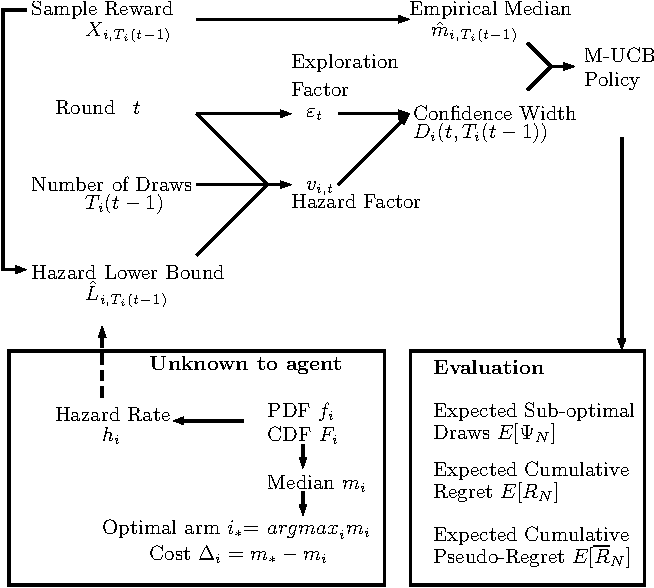
\includegraphics[scale=0.7]{plots/dependency_diagram.pdf}
    \caption{Summary of notation and the dependency between concepts in this paper.
    The variables on the heads of an arrow (i.e. the arrow point to) depend on those at the tails of the same arrow.
    %The bottom box includes information about the reward distributions of arms, which are unknown to the agent and used for evaluations.
    %The lower bound of the hazard rate is accessible to the agent.
    %The right box shows the evaluation methods.
    }
    \label{fig: Dependency Diagram of HazardUCB}
\end{figure}


The main assumption that enables the analysis in the following section is the following.
\begin{ass}
\label{ass:IHR}
The reward distributions have \emph{non-decreasing hazard rate (IHR)} with support $[0, \infty)$, i.e. for all $x_1, x_2 \in \mathbb{R}$ and $x_1 \geq x_2 \geq 0$, the hazard rate satisfies $h(x_1) \geq h(x_2)$.
\end{ass}
While the analysis of many other bandit algorithms require bounded support of the reward distribution \cite{Auer2002, audibert2009exploration, cassel_general_2018}, Assumption 1 allows reward distributions with unbounded support, i.e. $[0,\infty)$.
Refer to \cite{boucheron2012} for more details about the IHR assumption.
Recall the definition of a hazard rate (Definition~\ref{defi: Hazard Rate}).
If the hazard rate $h(T)$ increases as time goes by, the probability of the failure event happens in next $\Delta t$ will increase as $T$ increases, given an item has survived up to time $T$.
For example, a man is more likely to die within the next month when he is 88 years old than he is 18 years old.
The increasing (or non-decreasing) hazard rate (IHR) property reflects the most natural life pattern that one would wear out with time.
Many distributions have a non-decreasing hazard rate, including Gaussian, Exponential, Gumbel, and Logistic distribution.
Note that distributions with increasing hazard rate property is light-tailed distributions \cite{rinne_hazard_nodate}, which have thinner tails than an exponential distribution.
The IHR assumption enables us to derive bounds on $\sd$ and also regret bounds.
The form of the confidence width $D_i(t, T_i(t-1))$
in Algorithm~\ref{alg:Policy for IHR distributions} is chosen to exploit the IHR assumption.


\subsection{Tail Bounds for Empirical Medians}
\label{sec: Theorem}

%A nonasymptotic concentration inequality provides an upper bound on the probability that a random variable deviates from its expected value. In other words,

In this section, we justify our choice of confidence width, $D_i(t, T_i(t-1))$, in
Algorithm~\ref{alg:Policy for IHR distributions} by deriving logarithmic upper bounds
on the number of sub-optimal draws and expected regret.
We seek the upper bounds for
tail probabilities of the empirical median, $\hat{m}_{i,T_i(t-1)}$,
for each arm $i \in \mathcal{K}$ at round $t$
\begin{align}
\label{equ: general form of concen ine for medians}
    \mathbb{P}\left(\hat{m}_{i,T_i(t-1)}- \mathbb{E}[\hat{m}_{i,T_i(t-1)}] \geq D_i\left(t, T_i\left(t-1\right)\right)\right) \leq \delta_t,
\end{align}
where $\delta_t$ decreases as $t$ increases.

\iffalse
\begin{enumerate}[i]
    \item How a concentration inequality shown in (\ref{equ: general form of concen ine for medians}) can be derived based on Theorem \ref{theo: Exponential Efron-Stein inequality}?
    \item How well M-UCB performances in theory?
\end{enumerate}
\fi

Notation for concentration bounds (Section \ref{subsec: Bounding the space between order statistics} and \ref{subsec: concentration inequalities for medians}) applies to all arms $i \in \mathcal{K}$ and thus we suppress the index $i$,
i.e. instead of denoting $X_{i,1}, ..., X_{i,T_i(t-1)}$, we denote $X_{1}, ..., X_{n}$ as independently distributed according to a distribution $F$, where $n = T_i(t-1)$ is the number of samples for arm $i$ up to round $t-1$.
And let $X_{\left(1\right)} \geq \ldots \geq X_{\left(n\right)}$ be the order statistics.

Our concentration inequality is based on a recent result called the
Exponential Efron-Stein inequality \cite{boucheron2012} (Theorem \ref{theo: Exponential Efron-Stein inequality}).
We use this to bound the gap, $S_{k} = X_{\left(k\right)}-X_{\left(k+1\right)}$,
between order statistics in Section~\ref{subsec: Bounding the space between order statistics}.
We prove in Section~\ref{subsec: concentration inequalities for medians}
a Bernstein inequality on the difference
between the empirical $q$-quantile $X_{(qn)}$ and its expectation (Theorem~\ref{theo: Bernstein Inequality for Quantiles.}).
This enables us to prove a logarithmic bound
on expected sub-optimal draws (Section~\ref{subsec: Bounding the Sub-optimal Draws})
and expected regret (Section~\ref{subsec: Bounding the Regret}),
which is consistent with the state of the art.

\subsubsection{Bounding Space between Order Statistics}
\label{subsec: Bounding the space between order statistics}

%The gap between the Exponential Efron-Stein inequality (Theorem \ref{theo: Exponential Efron-Stein inequality}) and what we need to derive a confidence width term is that
%In Theorem \ref{theo: Exponential Efron-Stein inequality}, the upper bound of logarithm moment generating function of $X_{\left(k\right)}-\mathbb{E}[X_{\left(k\right)}]$ contains the expectation of space between order statistics, which leads to the existence of expectation in the confidence width term as well. However, the expectation is taken in terms of the reward distribution, which is not accessible by agents in the process of the game.


Theorem \ref{theo: Exponential Efron-Stein inequality} bounds the logarithmic moment generating function of $X_{\left(k\right)}-\mathbb{E} X_{\left(k\right)}$ with the exponential moments of the $k^{th}$ spacing $S_{k}$.
We derive a bound (Lemma~\ref{lemma: bound the upper bound of expon efron-stein})
for the right-hand side of Theorem \ref{theo: Exponential Efron-Stein inequality}
that will enable us to derive a bound for quantiles in the next section.

\begin{theo} [\textit{Exponential Efron-Stein inequality, Theorem 2.9 in \cite{boucheron2012}}]
\label{theo: Exponential Efron-Stein inequality}
Let $X_{\left(1\right)} \geq X_{\left(2\right)} \geq ... \geq X_{\left(n\right)}$ denote the order statistics of $X_1, ..., X_n$, and let $S_{k} = X_{\left(k\right)}-X_{\left(k+1\right)}$ be the $k^{th}$ spacing. For $\lambda \geq 0, 1 \leq k \leq n / 2$,
\begin{align}
    \label{equ: Exponential Efron-Stein inequality}
    \log \mathbb{E}[ e^{\lambda\left(X_{\left(k\right)}-\mathbb{E}[ X_{\left(k\right)}]\right)}]
    \leq \lambda \frac{k}{2} \mathbb{E}\left[S_{k}\left(e^{\lambda S_{k}}-1\right)\right].
\end{align}
\end{theo}

This upper bound contains an expectation taken with respect to the distribution $F$,
i.e. the reward distribution of each arm.
Since the reward distributions are unknown to agents, we cannot make use of this information to design our policies. So we need to further bound this inequality to avoid having expectations in the upper bound.
%With the assumption of non-decreasing hazard rate, we further bound this inequality for the UCB policy design in Section \ref{subsec: Bounding the space between order statistics}. We show the background of the hazard rate in the next section.
By assuming a non-decreasing hazard rate (Assumption~\ref{ass:IHR}),
we bound the term in right hand side of Exponential Efron-Stein inequality $\mathbb{E}\left[S_{k}\left(e^{\lambda S_{k}}-1\right)\right]$
in Lemma \ref{lemma: bound the upper bound of expon efron-stein}.
%Observe that the expectation in upper bound of Exponential Efron-Stein inequality is taken for a term containing $S_{k}$, following similar proof structure, we bound right-hand side of Exponential Efron-Stein inequality.


\begin{restatable}{lemma}{BoundUpperExpEfronStein}
\label{lemma: bound the upper bound of expon efron-stein}
Let $S_{k} = X_{\left(k\right)}-X_{\left(k+1\right)}$ be the $k^{th}$ spacing of order statistics, and the lower bound of hazard rate be $L$. Define $v_n = \frac{n}{k^2 L^2}$, for all $ 1 \leq k \leq \frac{n}{2},$
%the logarithmic moment generating function of $X_{(k)} - \mathbb{E}[X_{(k)}]$ in Theorem \ref{theo: Exponential Efron-Stein inequality} can be bounded with the assumption of IHR.
and all $\lambda$ such that $0 \leq \lambda< \frac{1}{2} \sqrt{\frac{n}{v_n}}$, we can bound $\lambda \mathbb{E}\left[S_{k}\left(e^{\lambda S_{k}}-1\right)\right]$ under Assumption \ref{ass:IHR} as following,
\begin{align}
\label{equ: bound the right hand side of EES}
    \lambda \mathbb{E}\left[S_{k}\left(e^{\lambda S_{k}}-1\right)\right] \leq
    \frac{2 \lambda^{2} v_{n} }{n\left(1-2 \lambda \sqrt{\frac{v_{n}}{n}}\right)}.
\end{align}
\end{restatable}

In Proposition \ref{prop: bound of expected spacing}, we show the expected space between order statistics can be bounded in terms of the index of space and the lower bound of hazard rate, which will not be used further in this paper, but can be useful for applications of order statistics.


\begin{restatable}{prop}{BoundExpSpacing}
\label{prop: bound of expected spacing}
Let $S_{k} = X_{\left(k\right)}-X_{\left(k+1\right)}$ be the $k^{th}$ spacing, and $L$ be the lower bound of hazard rate of distribution $F$. For any $1 \leq k \leq \frac{n}{2}$, the expectation of spacing $S_k$ can be bounded under Assumption \ref{ass:IHR},
\begin{align}
    \mathbb{E}[S_k] \leq \frac{1}{kL}.
\end{align}
\end{restatable}

The proof of Lemma \ref{lemma: bound the upper bound of expon efron-stein} and Proposition \ref{prop: bound of expected spacing} relies on R\`enyi's representation, see Appendix \ref{app-sec: Proof} for details.

%With the assumption of non-decreasing hazard rate (IHR) of the reward distributions, the expectation of space between order statistics can be bounded in terms of the lower bound of hazard rate. Lemma \ref{lemma: bound the upper bound of expon efron-stein} shows the right-hand side of Exponential Efron-Stein inequality in Theorem \ref{theo: Exponential Efron-Stein inequality} can be further bounded into a Bernstein-type formula.

\subsubsection{Bernstein Inequality for Quantiles}
\label{subsec: concentration inequalities for medians}

\begin{table*}[!ht]
\renewcommand{\arraystretch}{2}
\centering
\scalebox{0.9}{
\begin{tabular}{|c|c|c|c|}
\hline
& Arbitrary IHR Distribution & Absolute Centred Gaussian Distribution & Exponential Distribution  \\ \hline
$L_{i}$       & $L_{i}$  &   $\frac{1}{\sigma_i \sqrt{2 \pi}}$     &   $\theta_i$   \\ \hline
$\sd$ & $\sum_{i \neq i_\ast} \frac{ C_{i} \log N}{(\Delta_i L_{i})^2}  + 1 + \frac{\pi^2}{3}$   & $\sum_{i \neq i_\ast} \frac{2 \pi \sigma^2_i  C_{i} \log N}{\Delta_i^2}  + 1 + \frac{\pi^2}{3}$       &   $\sum_{i \neq i_\ast} \frac{ C_{i} \log N}{(\Delta_i \theta_{i})^2}  + 1 + \frac{\pi^2}{3}$   \\ \hline
$\mathbb{E}[R_N]$ &  $\sum_{i \neq i_\ast}\frac{ C_{i} \log N}{\Delta_i L_{i}^2}  + \xi$ & $\sum_{i \neq i_\ast} \frac{2 \pi \sigma^2_i  C_{i} \log N}{\Delta_i}  + \xi$ & $\sum_{i \neq i_\ast} \frac{ C_{i} \log N}{\Delta_i \theta_{i}^2}  + \xi$ \\ \hline
$C_{i}$ & $(2 + \Delta_i L_{i}) + 2\sqrt{1 +  \Delta_i L_{i}}$  & $(2 + \frac{\Delta_i}{\sigma_i \sqrt{2 \pi}} ) + 2\sqrt{1 + \frac{\Delta_i}{\sigma_i \sqrt{2 \pi}}}$ & $(2 + \Delta_i \theta_{i}) + 2\sqrt{1 +  \Delta_i \theta_{i}}$ \\ \hline
\end{tabular}
}
\caption{Expected sub-optimal draws and regret bound for special case distributions, where $C_{i}$ is shown in the last row, and $\xi = \left(1 + \frac{\pi^2}{3}\right) \left(\sum_{j=1}^K \Delta_{j}\right)$. See Appendix \ref{app-sec: special case} for definitions of special case distributions. }
\label{table: Summary for policies and bounds.}
\end{table*}


%Lemma \ref{lemma: bound the upper bound of expon efron-stein} extends Theorem \ref{theo: Exponential Efron-Stein inequality} into an inequality where upper bound does not include expectation.
For a bandit setting, it is more interesting to consider a percentage of distribution, i.e. empirical quantile $X_{(qn)}$ than a specific order statistics $X_{(k)}$.
With q-quantile as $\mathbb{E}[X_{(qn)}] = \inf \{x \in \mathbb{R} : q \leq F\left(x\right)\}$ (assume $qn$ is an integer), we derive a Bernstein like inequality for quantiles in Theorem \ref{theo: Bernstein Inequality for Quantiles.}, which resembles the Bernstein inequality (Theorem \ref{theo: Bernstein Inequality} in Appendix \ref{sec: Comparison with Related Work}).

%We show the concentration inequality for quantile in Theorem \ref{theo: Bernstein Inequality for Quantiles.}, since it exhibits a form of Bernstein inequality, we call it Bernstein inequality for Quantiles. As a special case for quantiles, we show the concentration inequality of medians in Corollary \ref{theo: Bernstein Inequality for Medians.}.
%We show how we bound the Exponential Efron-Stein inequality further in Theorem \ref{theo: Bernstein Inequality for Medians.}.

%------------------------------------------------------


\begin{restatable}[Bernstein Inequality for Quantiles]{theo}{BernQuant}
\label{theo: Bernstein Inequality for Quantiles.}
Let $X_{\left(1\right)} \geq X_{\left(2\right)} \geq ... \geq X_{\left(n\right)}$ denote the order statistics of $X_1, ..., X_n$, and $X_{(qn)}$ is the empirical $q$-quantile (assume $qn$ is an integer, $q \in (0, \frac{1}{2}]$).
Define $v_n = \frac{1}{q^2 n L^2}$, with Assumption \ref{ass:IHR},
for all $\lambda$ such that $0 \leq \lambda< \frac{1}{2} \sqrt{\frac{n}{v_n}}$,
\begin{align}
    \label{equ: log mgf for quantile}
    \log \mathbb{E}\left[e^{\lambda\left(X_{\left(qn\right)}-\mathbb{E}[X_{\left(qn\right)}] \right)}\right] \leq  \frac{\lambda^{2}  v_{n}}{2 \left(1-2 \lambda \sqrt{\frac{v_{n}}{n}}\right)}.
\end{align}
For all $\varepsilon > 0$, we obtain the concentration inequality
\begin{align}
    \label{equ: bernstein ineq for quantile}
    \mathbb{P}\left(X_{\left(qn\right)}-\mathbb{E}[X_{\left(qn\right)}] \geq \sqrt{2 v_{n} \varepsilon}+2 \varepsilon \sqrt{\frac{v_{n}}{n}}\right) \leq e^{-\varepsilon}.
    %\label{inequality Bernstein lower bound for abr}
    %\mathbb{P}\left\{\mathbb{E}[X_{\left(qn\right)}] - X_{\left(qn\right)}\geq \sqrt{2 v_{n} \varepsilon}+2 \varepsilon \sqrt{\frac{v_{n}}{n}}\right\} \leq e^{-\varepsilon}.
\end{align}
%where the expectation is taken with respect to the randomness of the environment.
\end{restatable}

\begin{proof-sketch}
By chaining the inequalities,
Equation~\eqref{equ: Exponential Efron-Stein inequality} from Theorem~\ref{theo: Exponential Efron-Stein inequality}, and
Equation~\eqref{equ: bound the right hand side of EES} from Lemma~\ref{lemma: bound the upper bound of expon efron-stein},
we obtain a new upper bound for the logarithmic moment generating function of $X_{(k)} - \mathbb{E}[X_{(k)}]$.
To express empirical quantiles, we replace $k$ with $qn$, and therefore substitute
$v_n = \frac{n}{k^2 L^2}$ with $v_n = \frac{1}{q^2 n L^2}$. Since $q \in (0, \frac{1}{2}]$, we have
$\frac{qn}{2} \times \frac{2 \lambda^{2} v_{n} }{n\left(1-2 \lambda \sqrt{\frac{v_{n}}{n}}\right)}
\leq \frac{\lambda^{2}  v_{n}}{2 \left(1-2 \lambda \sqrt{\frac{v_{n}}{n}}\right)}.$
Thus we obtain (\ref{equ: log mgf for quantile}).
Then choose a value of $\lambda$ which minimises the upper bound of (\ref{equ: log mgf for quantile}) and based on the Cram\'er-Chernoff method \cite{boucheron2013}, (\ref{equ: bernstein ineq for quantile}) is proved.
For whole proof, see Appendix \ref{app-sec: proof for theo: Bernstein Inequality for Quantiles.}.
\end{proof-sketch}


%Intuitively, since the hazard rate is non-decreasing, the expectation of space between order statistics should be smaller then the time goes by (i.e. k increases). And the largest the spacing is still bounded by the lower bound of the hazard rate. We will make use of this interesting pattern to bound the Exponential Efron-Stein inequality in Theorem \ref{theo: Bernstein Inequality for Quantiles.}.
A special case for Theorem \ref{theo: Bernstein Inequality for Quantiles.} is when $q = \frac{1}{2}$, we have the concentration inequality for medians.

\begin{coro}[Bernstein Inequality for Medians]
\label{theo: Bernstein Inequality for Medians.}
Let $X_{\left(1\right)} \geq X_{\left(2\right)} \geq ... \geq X_{\left(n\right)}$ denote the order statistics of $X_1, ..., X_n$,
and $\hat{m} = X_{(\frac{n}{2})}$ be the empirical median. Define $v_n = \frac{4}{n L^2}$, with Assumption \ref{ass:IHR}, for all $\varepsilon > 0$,
\begin{align}
\label{equ: inequality Bernstein bound for median}
    \mathbb{P}\left( \hat{m}-\mathbb{E}[\hat{m}] \geq \sqrt{2 v_{n} \varepsilon}+2 \varepsilon \sqrt{\frac{v_{n}}{n}}\right) \leq  e^{-\varepsilon}.
\end{align}
%where the expectation is taken with respect to distribution $F$.
\end{coro}

Observe that the term $\sqrt{2 v_{n} \varepsilon}+2 \varepsilon \sqrt{\frac{v_{n}}{n}}$ in the inequality (\ref{equ: inequality Bernstein bound for median}) provides the confidence width term in Algorithm \ref{alg:Policy for IHR distributions} with $n = T_i(t-1)$, $v_n = v_{i,T_i(t-1)}$ (we denote as $v_{i,t}$ in Section \ref{sec: policy} for simplicity), and $\varepsilon = \varepsilon_t$.
%parameters adapting to the bandit setting.

\subsubsection{Bounding the Sub-optimal Draws}
\label{subsec: Bounding the Sub-optimal Draws}

M-UCB is designed to minimise the expected number of sub-optimal draws $\sd$
(Definition \ref{defi: sub-optimal draws}) up to round $N$.
We show in Theorem~\ref{theo: sub-optimal draws bound} that the expected number
of sub-optimal draws $\sd$ is bounded by a logarithmic rate,
and show the proof in the Appendix~\ref{app-subsec: proof of theo: sub-optimal draws bound}. Recall that we define the optimal arm $i_\ast = \argmax_{i \in \mathcal{K}} m_i$, and $m_i, m_\ast$ as the median of arm $i$ and the optimal arm respectively. We show the proof for the case where $\alpha = 4, \beta =1$ in M-UCB policy.

\begin{restatable}[Sub-optimal draws bound]{theo}{SubOptDrawsBound}
\label{theo: sub-optimal draws bound}
Let $\Delta_i$ be the difference between median of the optimal arm and arm $i$,
i.e. $\Delta_{i} = m_\ast - m_i$, and $L_i$ be the lower bound of hazard rate for arm $i$.
For all K $>$ 1, if the proposed policy M-UCB is run on K arms with reward distributions under Assumption \ref{ass:IHR},
%$$h\left(U\left(exp\left(y\right)\right)\right) = \frac{f\left(U\left(exp\left(y\right)\right)\right)}{\bar{F}\left(U\left(exp\left(y\right)\right)\right) } \geq L,$$
%where $\bar{F} = 1 - F$, R-transform is defined in Definition \ref{defi: R-transform}, $y > 0$, $L > 0$.
then the upper bound of the expected sum of sub-optimal draws $\sd$  at round $N$
is given by
%Cheng: I don't see where you need $\varepsilon$
%More precisely, when set $\varepsilon = 4 \log t$,
\begin{align}
    \sd \leq \sum_{i \neq i_\ast} \frac{ C_{i} \log N}{(\Delta_i L_{i})^2}  + 1 + \frac{\pi^2}{3},
\end{align}
where $C_{i} = 32[(2 + \Delta_i L_{i}) + 2\sqrt{1 +  \Delta_i L_{i}}]$. %$\pi$ is the mathematical constant.
\end{restatable}

\begin{proof-sketch}
Arm $i$ is selected at round $t$ (i.e. $A_t = i$) only when the upper confidence width for arm $i$ constructed by M-UCB (i.e. $\hat{m}_{i, T_i\left(t-1\right)} +  D_i\left(t, T_i\left(t-1\right)\right)$) is larger than or equal to the one for the optimal arm. 
%Define  $l' = \Bigl\lceil \frac{C_{i} \log N}{(\Delta_i L_{i})^2}  \Bigr\rceil,$ and set $\alpha = 4, \beta = 1$, from Lemma \ref{lemma: upper bound of expected number of draws} in Appendix \ref{app-subsec: proof of theo: sub-optimal draws bound}, 
For a particular choice of $l'$, $0 < s <t$, and $l' \leq s_i <t$ (see Lemma 3 and 4 for details), we can decompose the probability of choosing the arm $i$, 
\begin{align}
    & \mathbb{P}\left(\hat{m}_{*, s} +  D_*(t, s)  \leq \hat{m}_{i, s_i} +  D_i(t, s_i)\right) \nonumber \\
    \leq &  \mathbb{P}\left(\hat{m}_{*, s} +  D_*(t, s) \leq  \mathbb{E}[\hat{m}_{*, s}]\right) + \nonumber \\ & \mathbb{P}\left(\hat{m}_{i, s_i} -  D_i(t, s_i) \geq \mathbb{E}[\hat{m}_{i, s_i}]\right).
\end{align}
For non-negative distributions, the two-side version of Corollary \ref{theo: Bernstein Inequality for Medians.} can be proved 
\begin{align}
        & \mathbb{P}\left(\hat{m}_{*, s} +  D_*(t, s) \leq  \mathbb{E}[\hat{m}_{*, s}]\right) \nonumber\\ 
\label{equ: lower side of bernstein inequality for median}
        \leq & \mathbb{P}\left(\hat{m}_{i, s_i} -  D_i(t, s_i) \geq \mathbb{E}[\hat{m}_{i, s_i}]\right)
        \leq   e^{- \varepsilon}.
    \end{align}
Note that the bound (\ref{equ: lower side of bernstein inequality for median}) is not sharp. 
We take an expectation of $T_i(t-1)$ 
%(recall Definition \ref{defi: sub-optimal draws})
to obtain a bound on the expected number of draws in terms of Corollary \ref{theo: Bernstein Inequality for Medians.}.
The whole proof is shown in Appendix \ref{app-subsec: proof of theo: sub-optimal draws bound}.

\end{proof-sketch}


\subsubsection{Bounding the Regret}
\label{subsec: Bounding the Regret}

To enable comparison with other bandit algorithms, we now
%The expected regret bound can be derived based on $\sd$.
%The regret is the cost we need to pay because we do not know the optimal arm ahead.
introduce the median-based regret and pseudo-regret,
and show in Proposition~\ref{prop: expectation of regret and pseudo-regret for median}
that they are in fact equivalent.


%Instead of summing up the sup-optimal draws, we consider the weighted sum of sup-optimal draws, where the weights are specified by the cost of choosing arm $i$ instead of choosing the optimal arm.

\begin{defi}[Median-based Regret]
\label{defi: regret for median}
The median-based regret is defined as 
%the difference between the sum of empirical medians under the optimal policy (i.e. always choosing the optimal arm) and the sum of empirical medians under M-UCB policy.
\begin{align}
    & R_N = \sum_{t=1}^N \hat{m}_{\ast, t} - \sum_{t = 1}^N \sum_{i = 1}^K \hat{m}_{i, T_i(t)} \mathbb{I}\{A_t = i\}.
\end{align}
\end{defi}

\begin{defi}[Median-based Pseudo-regret]
\label{defi: pseudo-regret for median}
The median-based pseudo-regret is defined based on the medians of arms.
    \begin{align}
    & \overline{R}_N = N m_\ast - \sum_{i=1}^K m_i T_i(N).
        %\mathbb{E}[\overline{R}_N] = \sum_{i = 1}^K \Delta_{i} \mathbb{E}[T_i\left(N\right)],
    \end{align}
\end{defi}

By taking medians of sample rewards at each round, the median-based regret reflects the difference of the cumulative empirical median between the M-UCB policy and the optimal policy. Similar as risk-averse regret (see Appendix \ref{app-subsec: Risk-averse Regret} for an example),
%the difference between the median-based regret and the mean-based regret (inequality \ref{equ: mean based regret}) is that
minimising the median-based regret is not equivalent to maximising the cumulative rewards.

\begin{restatable}{prop}{EquMedianRegret}
\label{prop: expectation of regret and pseudo-regret for median}
The expectations of median-based regret and pseudo-regret defined in Definition \ref{defi: regret for median} and \ref{defi: pseudo-regret for median} are equivalent and can be decomposed into the weighted sum of sub-optimal draws.
i.e. $\mathbb{E}[R_N] = \mathbb{E}[\overline{R}_{N}] = \sum_{i=1}^K \Delta_i \mathbb{E}[T_i(N)]$,
where $\Delta_i = m_\ast - m_i$.
\end{restatable}

Bounding the expected median-based regret is equivalent to
%bounding the expected median-based pseudo-regret, which is also equal to
bounding the expected number of sub-optimal draws.
Recall from Definition~\ref{defi: sub-optimal draws} that $\Psi_N$ is
directly related to the number of draws $T_i(N)$, and hence
the expected regret bound can be derived based on
Proposition~\ref{prop: expectation of regret and pseudo-regret for median} and
Theorem~\ref{theo: sub-optimal draws bound}

\begin{restatable}[Regret bound]{coro}{RegretBound}
\label{theo: regret bound}
Let $L_i$ be the lower bound of hazard rate, and $\Delta_i$ be the difference between median of the optimal arm and arm $i$, i.e. $\Delta_{i} = m_\ast - m_i$.
For all K $>$ 1, if the proposed policy M-UCB is run on K arms with reward distributions under Assumption \ref{ass:IHR},
then the upper bound of the expected regret $\mathbb{E}[R_N]$ is given by
% Cheng: I don't see \varepsilon anywhere in this theorem
%More precisely, when set $\varepsilon = 4 \log t$,
\begin{align}
    \label{equ: regret bound}
    \mathbb{E}[R_N] \leq \sum_{i \neq i_\ast}\frac{C_{i} \log N}{\Delta_i L_{i}^2}  + \left(1 + \frac{\pi^2}{3}\right) \left(\sum_{j=1}^K \Delta_{j}\right) ,
\end{align}
where $C_{i} = 32 \left[(2 + \Delta_i L_{i}) + 2\sqrt{1 + \Delta_i L_{i}}\right]$.
%$\pi$ is the mathematical constant.
\end{restatable}

We show the bound on expected sub-optimal draws and expected regret for the general case and two special cases: absolute centred Gaussian distribution and exponential distribution in Table \ref{table: Summary for policies and bounds.}. 
%The definition of two special cases can be found in Appendix~\ref{app-sec: special case}.

\textbf{Regret Design Discussion:} The definition of regret depends on the choice of summary statistics for reward distributions.
When defining the optimal arm as the one with the highest mean, the mean-based regret and pseudo-regret are defined as \cite{Auer2002},
\begin{align}
    \label{equ: mean based regret}
    R^\mu_{N} &= \sum_{t=1}^{N} X_{\ast, t}-\sum_{t=1}^{N} \sum_{i = 1}^{K} X_{i, T_i(t)} \mathbb{I}\{A_t = i\},\\
    \label{equ: mean based pseudo regret}
    \overline{R}^\mu_{N} &=
    N \mu^{*}-\sum_{t=1}^{N} \sum_{i = 1}^{K} \mu_i \mathbb{I}\{A_t = i\},
\end{align}
where $X_{\ast, t}$ is the sample reward from the optimal arm at round $t$, and $\mu^\ast, \mu_i$ are the mean of optimal arm and arm $i$.
Minimising the mean-based regret is equivalent to maximising the cumulative reward.
The expected mean-based regret and pseudo-regret are equal and can be decomposed into the weighted sum of sub-optimal draws, i.e.  $\mathbb{E}[R^\mu_N] = \mathbb{E}[\overline{R}^\mu_{N}] = \sum_{i=1}^K \Delta^\mu_i \mathbb{E}[T_i(N)]$, where $\Delta^\mu_i = \mu_\ast - \mu_i$.


When evaluating distributions by different summary statistics, regret can be defined accordingly. For example,  \textcite{cassel_general_2018} evaluates performance by means of a function $U$, which maps the empirical distribution $\hat{F} \text { to } \mathbb{R}$. Correspondingly, a risk-averse regret is proposed as the difference between $U$ measure of average empirical distributions with the optimal policy and their policy. Similarly, we define our regret as the difference between the medians of reward distributions.
More discussion about different notions of regret can be found in Appendix \ref{app-sec: Design Choice of Regret}.
%--------------------------------------------------------------


\subsection{Empirical Evaluations}
\label{sec: Empirical Experiments}

We show the empirical performance of our policy on simulated data and two clinical treatment datasets\footnote{Implementation available at \url{http://hidden.url}}.
We compare our policy (\ourpolicy) with two mean-based algorithms (UCB1 \cite{Auer2002}, UCB-V \cite{audibert2009exploration}), one risk-averse algorithm MV-LCB \cite{sani_risk-aversion_2012} and one adversarial algorithm Exp3 \cite{Auer2003adv} in terms of expected sub-optimal draws and expected regret.
The Exp3 does not make assumptions about the reward distribution,
which might suit the outlier setting better.
%For each experiment, we show histograms of reward distributions in the first row, and report the expected sub-optimal draws and expected regret in the second and third-row respectively.

The optimal arm and regret are defined in accordance with the benchmark algorithms,
e.g. the optimal arm of UCB1 is the arm with the maximum mean,
and the regret is the mean-based regret (\ref{equ: mean based regret}).
See Appendix \ref{app-sec: Experiment Design and Report} for the details of benchmark algorithms.

The expected regret is not directly comparable for algorithms with different definitions of regret. The mean-based algorithms have the goal of maximising the cumulative reward, while risk-averse algorithms have the goal of minimising the risk or balancing the risk and reward.
This is why we show the expected sub-optimal draws, which is directly comparable. However
we also provide results for expected regret, to enable comparisons with other papers.

\subsubsection{Simulations}
\label{subsec: Simulations}

\begin{table}[t]
\scalebox{0.9}{
\begin{tabular}{|c|c|c|}
\hline
  Arms & No Outliers       & With Outliers                                                                               \\ \hline
A & $|\mathcal{N}(0, 0.5)|$ & $0.95 |\mathcal{N}(0, 0.5)| + 0.05 |\mathcal{N}(20, 0.5)|$\\ \hline
B & $|\mathcal{N}(0, 0.1)|$ & $0.95 |\mathcal{N}(0, 0.1)| + 0.05 |\mathcal{N}(20, 0.5)|$ \\ \hline
C & $Exp(1)$         & $0.95 Exp(1) + 0.05 |\mathcal{N}(20, 0.5)|$        \\ \hline
\end{tabular}
}
\caption{Simulated reward distributions for 3 arms. The reward distributions are absolute Gaussian and Exponential distribution (details in Appendix \ref{app-sec: special case}). }
\label{table: Simulated reward distributions for 3-arm setting.}
\end{table}

\begin{figure}[t]
    \centering
    %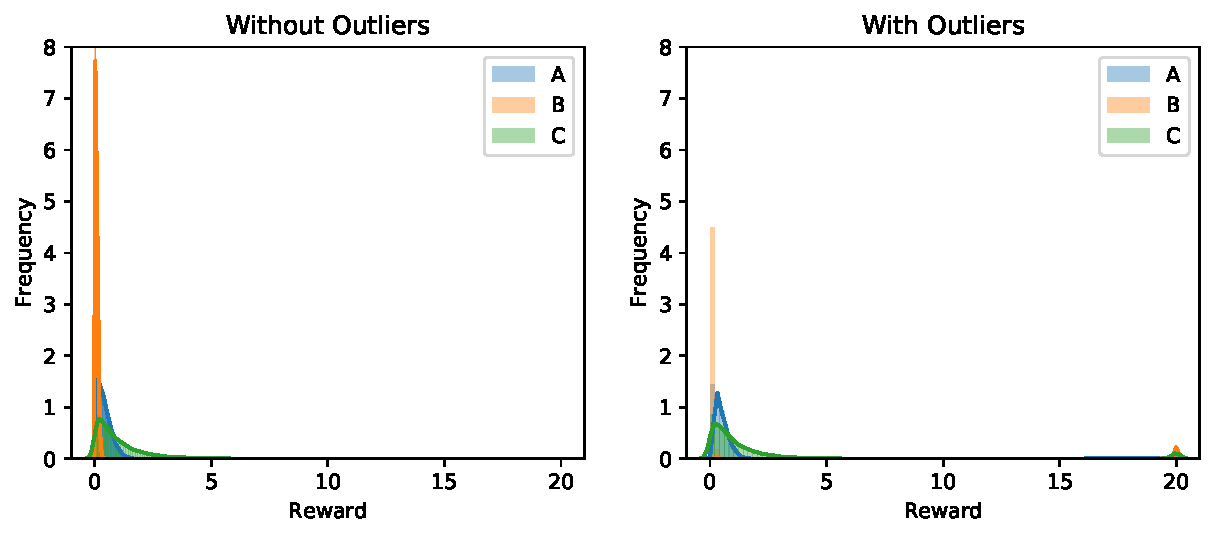
\includegraphics[scale=0.4]{plots/Hist.pdf}
    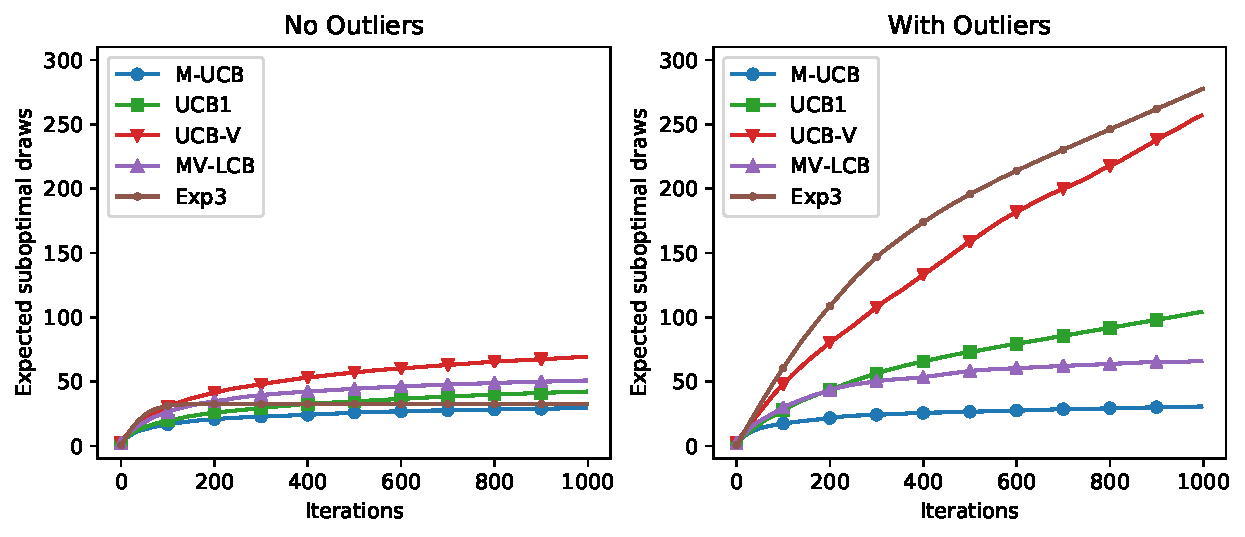
\includegraphics[scale=0.4]{plots/Exper_sd.pdf}
    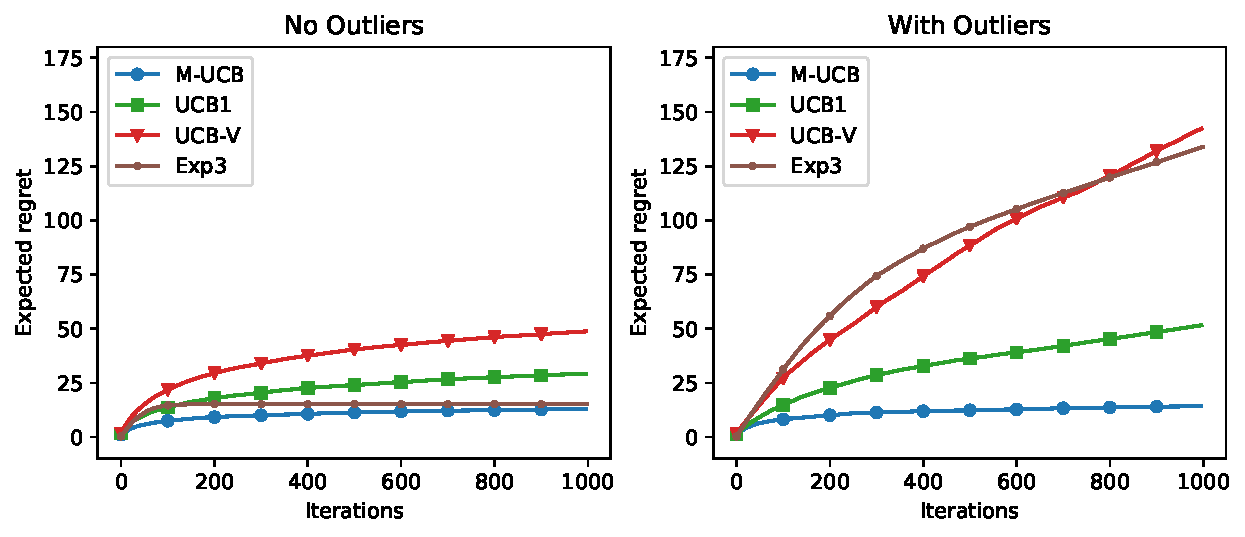
\includegraphics[scale=0.4]{plots/Exper_r.pdf}
    \caption{Simulation Experiment.% Top: Reward histogram.
    Top: Expected sub-optimal draws.
    Bottom: Expected regret (MV-LCB is too large and is not shown).
    M-UCB with parameter $\alpha = 0.5, \beta = 0.2$.
    }
    \label{fig: Simulated experiment.}
\end{figure}

We simulate 100 independent experiments, for a bandit task with 3 independent arms for
1000 rounds.
We consider two experimental settings, corresponding to two types of reward distributions:
with and no outliers, as summarised in
Table \ref{table: Simulated reward distributions for 3-arm setting.}.
The outliers are an absolute Gaussian centred at 20.

Figure \ref{fig: Simulated experiment.} shows that
M-UCB outperforms other methods
and has a stable performance for the situations with or without outliers,
in terms of both expected sub-optimal draws and expected regret.
Unsurprisingly, mean-based algorithms (UCB1 and UCB-V) are more sensitive to outliers
compared to the risk-averse MV-LCB and our algorithm \ourpolicy,
especially when the support of outliers is bigger than assumed reward support.
Surprisingly, the outliers also cause the adversarial algorithm Exp3 to have
worse performance. From the plot of the expected sub-optimal draws,
we observe that MV-LCB is robust to outliers but still has a larger number of sub-optimal
draws than \ourpolicy.

% Cheng: I'm removing this discussion because we don't show evidence of this in the experiments.
%The reason our algorithm has better performance is (1) Under the IHR assumption, our policy provides tighter upper confidence bound. (2) By using empirical medians to measure the rewards, our policy is robust to outliers. (3) Our policy does not assume bounded support, while other algorithms do. When the reward distribution is unknown, we may need to assume large support, and those algorithms will have a large number of sub-optimal draws.

%In figure \ref{fig: Example reward distributions.}, we have shown different estimators of the reward distributions can lead to a different order of the arm ranking. The medians estimators can better suit the risk-averse decision-makers. In this section, we show that even though different estimators have the same optimal arm, our policy still has a better performance for IHR distributions.



\subsubsection{Effect of Treatment on Cancer Survival}
\label{subsec: Real Data Experiments}

\begin{figure}[t]
    \centering
    \subfloat{{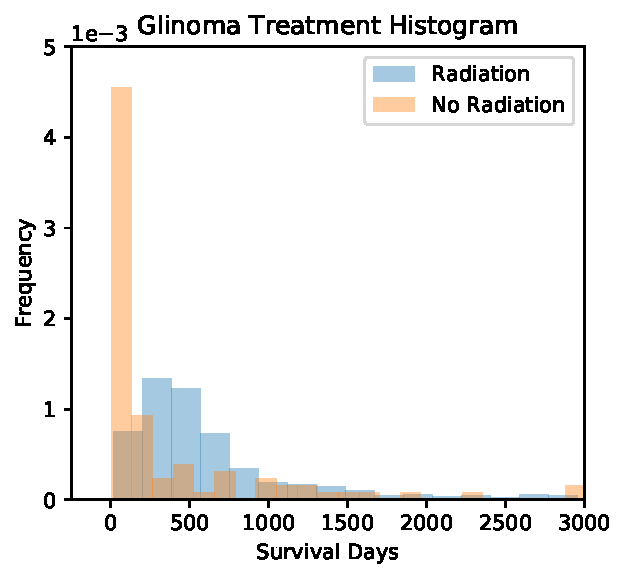
\includegraphics[scale = 0.38]{plots/glinoma_hist.pdf} }}%
    \subfloat{{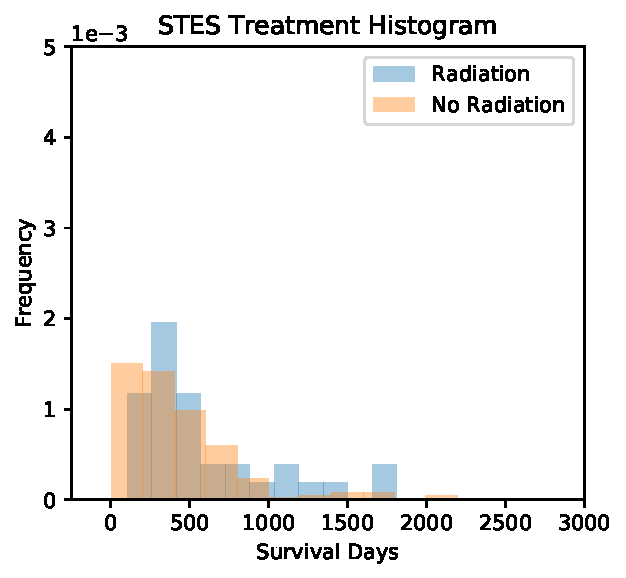
\includegraphics[scale = 0.38]{plots/STES_hist.pdf} }}\\
    \subfloat{{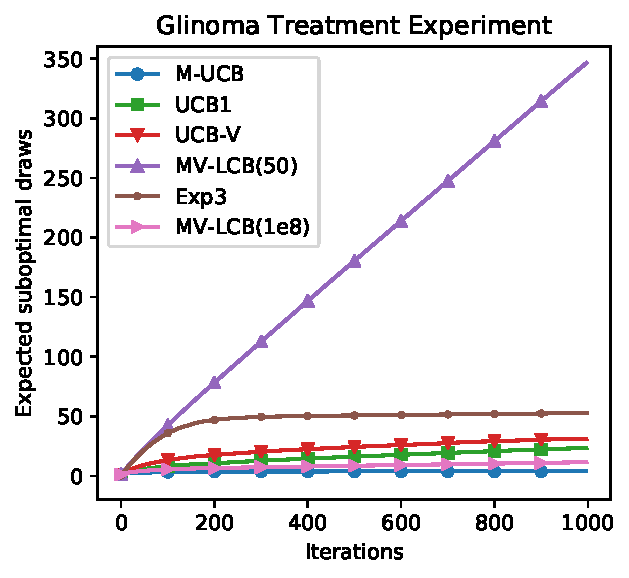
\includegraphics[scale=0.38]{plots/Glinoma_treatmet_sd.pdf} }}
    \subfloat{{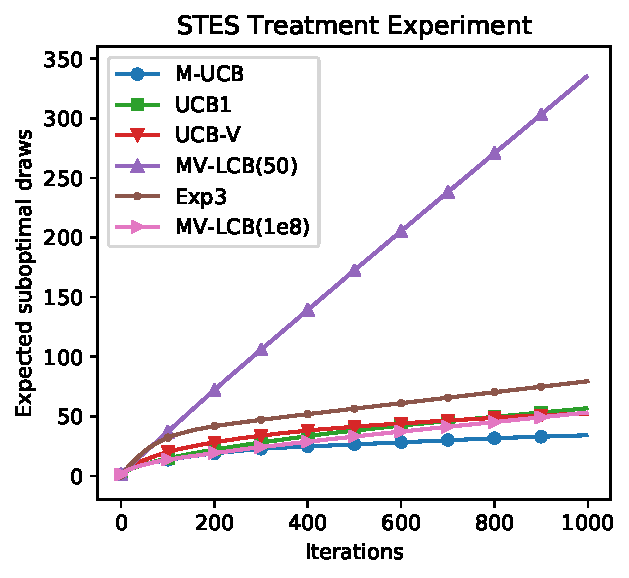
\includegraphics[scale=0.38]{plots/STES_treatmet_sd.pdf} }}\\
    \subfloat{{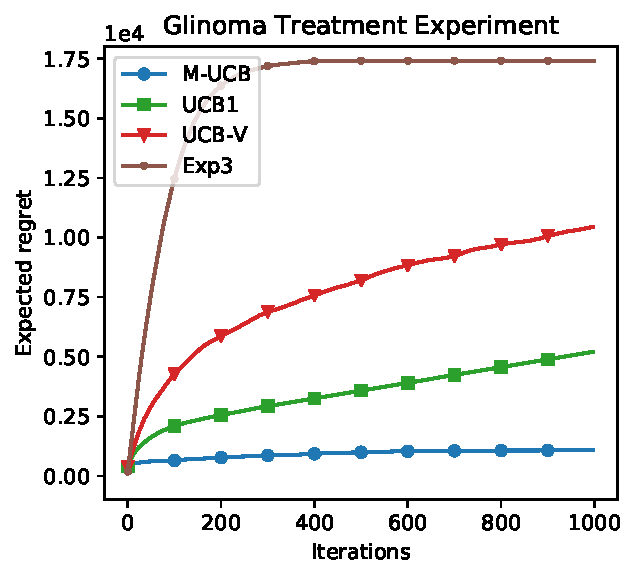
\includegraphics[scale=0.38]{plots/Glinoma_treatmet_r.pdf} }}
    \subfloat{{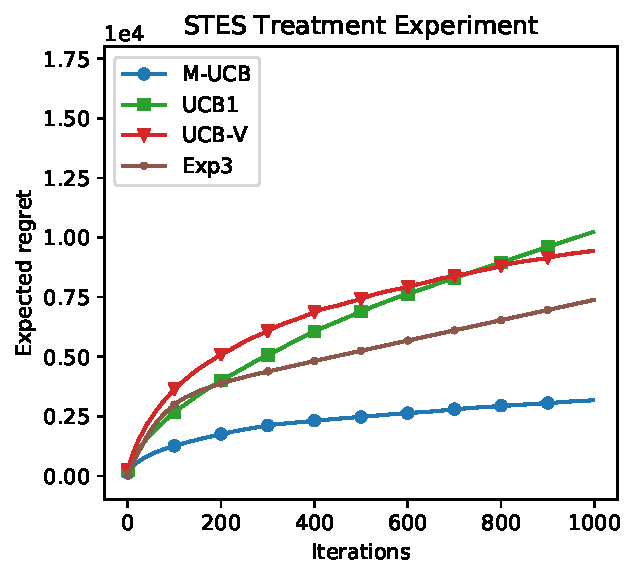
\includegraphics[scale=0.38]{plots/STES_treatmet_r.pdf} }}%
    \caption{ Clinical experiment. Top: Reward histogram.
    Middle: Expected sub-optimal draws.
    Bottom: Expected regret (MV-LCB is too large and is not shown).
    M-UCB with parameter $\alpha = 4, \beta = 1$.}
    \label{fig: Glinoma Clinical Treatment.}%
\end{figure}

The clinical experiment is a classical example of bandit problems. The type of treatments needs to be determined when patients arrive sequentially and the effectiveness of treatments are initially unknown \cite{thompson1933likelihood}.
Survival analysis with medians and hazard rate are commonly used in clinical experiment analysis \cite{panaphut_ceftriaxone_2003, panaput_dialysis_2014}.
The survival time reward distributions in such applications satisfy our IHR assumption.
Decision-makers in clinical treatments need to manage risk and maximise the optimal choices (i.e. minimise the number of sub-optimal choices).
Furthermore, empirical medians (the basis of our approach) are robust against outliers and positively skewed distributions.

We use two clinical datasets from Broad Institute Firehouse\footnote{\url{https://gdac.broadinstitute.org/}
}, namely the Glinoma dataset, and the Stomach and Esophageal carcinoma (STES) dataset.
These were chosen because they have a large number of samples.
For both datasets, there are two choices \textit{Radiation} and \textit{No Radiation},
and the reward is the number of days a patient survives (Survival Days).
As patients arrive sequentially, our goal is to minimise the sub-optimal treatment choices.
%There 588 valid records for the patient.

We repeat our experiment 500 times, each with 1000 rounds where we sample from
the database of records with replacement.
The reward distributions are positively skewed and have outliers in the right tail.
A small number of patients survived longer than 3000 days which are not shown in the histogram.
Our policy outperforms others in terms of both expected sub-optimal draws and regret, having a stable performance for both datasets.

For expected sub-optimal draws, we compare two parameter settings of MV-LCB.  When choosing a very large $\rho$ (1e8), MV-LCB policy evaluates empirical mean and has a similar form to UCB1. In this case, MV-LCB has a reasonably small expected sub-optimal draws, but it does not manage the risk control. When $\rho$ is small (50), MV-LCB has linear sub-optimal draws.
%--------------------------------------------------------------
\subsection{Summary}
\label{sec: Discussion}

In this paper, we proposed \ourpolicy, a policy that summarises the reward distribution
in terms of empirical median instead of the empirical mean.
This takes advantage of the robustness of medians,
allowing our policy to be robust to outliers and skewed distributions.
The main assumption required in the derivation of the new policy is that the reward
distributions have a non-decreasing hazard rate (Assumption \ref{ass:IHR}).
This assumption allows us to bound the spacing between order statistics
(Proposition \ref{prop: bound of expected spacing}) which leads to a bound using the
Exponential Efron-Stein inequality (Theorem \ref{theo: Exponential Efron-Stein inequality}).
Similar to other UCB style algorithms, our policy has two parts,
namely the empirical median and the confidence width.
Our confidence width is constructed from a Bernstein inequality for quantiles
(Theorem \ref{theo: Bernstein Inequality for Quantiles.}).
We proved a logarithmic upper bound of the expected sub-optimal draws $\sd$ and expected regret
$\mathbb{E}[R_N]$, which is consistent with the state of the art in bandit regret.
We demonstrated that M-UCB outperforms related policies on both simulated data and
a clinical treatment dataset.
We hope that this line of analysis will lead to a new class of bandit algorithms
which are based on order statistics, and are robust to outliers.



\section{Optimized Experimental Design for Translation Initiation using Machine Learning}

Synthetic Biology is on the verge of a leap into high-throughput data generation for which new methods of data handling and analysis will have to be developed. In this work, we show how machine learning can be used to analyse, predict the performance of the ribosome binding site (RBS) of E. coli – one of the main genetic elements controlling protein expression. We also show how to sequentially design the RBS sequence the find the optimal choice with high protein expression as fast as possible.  

We build a Gaussian process regression model to predict the translation initiation rate (TIR) of each gene in terms of different RBS design. We formalize sequential experiment design as a multiarmed bandit problem.  All possible unique sequences of RBS form the decision set, and the algorithm recommends design choices for each round. The experimental validation uses synthetic biology, with a plasmid inserted into E. coli. We compare our experimental design with random selections, in terms of the cumulative regret caused by not choosing the optimal sequence.

We have analysed a number of datasets available from literature guiding our choice of algorithms and encoding methods. We discuss the generation and analysis of custom data produced in the CSIRO-UQ BioFoundry.

Machine learning is seeing increasing use in synthetic biology, where it guides more and more design decisions. In this instance we have shown how Gaussian process regression model can be used for prediction of TIR of an E. coli RBS.




\chapter{Research Approaches} \label{chap-3}

\section{Research questions}

In the following, I list the ideas come to my head in two main groups, one is the extension of the current work M-UCB, one is for our current designing RBS project.  When more literature review is done, I plan to select two or three of them to attack and write detailed research methods proposal in later section. 

\subsection{M-UCB related}

\begin{enumerate}
    \item Whether can we design a bandit algorithm based on medians/quantiles with the objective function in best arm identification setting? i.e. consider M-UCB in BAI setting. There are two main objective functions to be considered: PAC (fixed confidence); sample complexity (fix budget). 
    
    \item Whether can we extend the M-UCB algorithm into a quantile version? what's the gap between M-UCB and a quantile-UCB?
    
    \item Whether can we extend the M-UCB algorithm into qualitative rewards? It makes sense since our concentration inequality is based on order statistics. If so, what's the difference for our approach compared with [Szorenyi et al 2015]. 
    
    \item Whether can we design a bandit algorithm based other summary statistics except quantile and mean? For example, it is interesting to consider coherent risk measures. CVaR could be a good start.
        \begin{itemize}
            \item figure out the literature have already achieved for CVaR bandit. Start from [Kagrecha et al 2019].
            \item Figure out other possibilities. e.g. Entropic value at risk, tail value at risk. 
            \item Figure the motivation of considering risk of bandit. Can it be a general interest? say, for example, is it interesting for finical applications? or can it be generalised to a MDP problem. 
            \item If it's a general interesting, then it would be great to consider a general framework for risk averse bandit. Similar idea can be referred to [cassel et al 2018].
        \end{itemize}
        
    \item Now we are considering sub-Gaussian or sub-exponential distributions for reward distributions. Can we consider a heavier tail distributions? For example, heavy-tailed distribution with finite $1 + \varepsilon$ moment, where $\varepsilon \in (0,1)$. One possible way to do that is to consider estimator of summary statistics [mean: Bubeck et al. 2013][CVaR: Kagrecha et al. 2019].
    
    \item Another way to think about new directions could be, what applications need bandits? what's the gap between we already can solve by bandit algorithms and what is required by the applications. One example is we need ordinal values for reward sometimes, so [Szorenyi et al 2015] proposed a quantile-based bandit. 
    \begin{itemize}
        \item List at lease three gaps (applications).
        \item Try to proposed the idea we can attack those gaps. (No detailed approaches needed).
    \end{itemize}
    
    \item Can we propose a quantile/CVaR based bandit algorithm assuming there are correlations between arms? A quantile/CVaR Bayesian regression algorihtm is a possible idea. Back to the idea that, if we consider GPUCB where the reward distribution for each arm which is not generated from a Gaussian distribution, not some general distribution, e.g. sub-Gaussian, or even heavier tails, how can we attack that problem?
    \begin{itemize}
        \item Figure out whether there are results for concentration inequality for quantile/CVaR regression. 
    \end{itemize}
    
\end{enumerate}

\subsection{Synthetic biology related}

\begin{enumerate}
    \item Embedding for sequences:
        \begin{itemize}
            \item Can we design a spectrum kernel with different weights for different pairs of letters? For example, A-T, C-G pairs should have higher weights since they are more similar. 
            
            \item Can we embedding sequences using BERT model? Similar idea was proposed for embedding protein. 
        \end{itemize}
    \item Can we analyse GPUCB in terms of fixed budget BAI objective, which is closer to our setting compared with the regret objective.
    \item What's other possible ideas to recommend arms in batch, instead of returning top n?
\end{enumerate}

\section{Research methods proposal}

\chapter{Work Plan} \label{ch-1}

\section{Research}

The future work for research is structured into 2 main parts.

\begin{enumerate}
    \item Similarities between Arms.\\
    First, based on the current research, I am interested in exploring the similarities between arms for bandits problems. Two directions for exploring this topic can go in parallel. 
    \begin{itemize}
        \item Extend the current work (Median-based UCB) to the graph/contextual setting.
        \item Using bandits to recommend DNA sequence for synthetic biology design.
    \end{itemize}
    
    \item Summary Statistics for Bandits.\\
    One interesting question is that, except median, what other summary statistics can be considered as summarising the reward distribution, and what kind of summary statistics suits for what the user requirements? For example, taking risk into consideration. Then whether we can derive a corresponding confidence width term in terms of these statistics?  
    
\end{enumerate}

The final goal is to consider different summary statistics for both independent and dependent arms in the bandit setting.



\section{Internship}

About: similarities between arms in bandits\\
Possible topic: graph bandits; contextual bandits\\
To be decided.

\section{Tutoring and Courses}

Tutoring List: Statistical Machine Learning.\\
Course List: Graph Course; Biology Course; Reinforcement Learning Course.

\section{Timeline}

I commenced my Ph.D. from 2018/8.

\begin{itemize}
    \item 2019/11 - 2020/2: \\
    SynBio with bandits algorithms with existing data (hopefully novelty in designing models for identifying similarity between arms, or in embedding sequences).\\
    Target: ICML (Deadline 2020/2/7)
    \item 2019/11 - 2020/5: \\
    Extend the M-UCB to contextual/graph bandit model (considering risk for contextual models).\\
    Target: NeuIPS (Deadline in May 2020)
    \item 2019/11 - 2020/6: \\
    SynBio with bandits algorithms with new data (hopefully help to identify some interesting biology properties) \\
    Target: Biology Journal (depends on how collaborators think)
    \item 2020/6 - 2020/12:\\
    2020/6/3 - 202/6/5: AISTATS (depends on whether get accepted)\\
    2020/6/12 - 2020/6/18: ICML2020\\
    2020/6/28 - 2020/7/10: MLSS in Germany\\
    2020/7 - : internship (to be decided, and hopefully one paper during internship)\\
    \item 2021/1 -2021/6:\\
    Depends on the research progress. But the current plan is to research on different summary statistics for bandits, for both dependent and independent arm cases. 
    Combine the AISTATS, NeurIPS, and summary statistics material into one paper.\\
    Target: JMLR
    
    
    
    
\end{itemize}

\chapter{Conclusion} 
 
%----------------------------------------------------------------------------------------

\clearpage
\printbibliography

\clearpage


%	APPENDICES
%----------------------------------------------------------------------------------------

\addtocontents{toc}{\vspace{2em}} % Add a gap in the Contents, for aesthetics
\appendix % Starts of appendices


\numberedchapter


\chapter{Supplementary material to \ourtitle} \label{appA}

\section{Regret Background}
\label{app-sec: Design Choice of Regret}

Depending on the design choice of the summary statistic of reward distributions, the regret can have different design choices.
In this section, we first show the background of regret design choice, namely the mean-based regret \cite{Auer2002, audibert2009exploration, garivier2011kl}, and the risk-averse regret (using the design choices of U-UCB \cite{cassel_general_2018} as an example), then we show the proof of our median-based regret. 
%For each choice, we define the regret and pseudo-regret, following by showing when their expectations are equal and the gap between them. Then we show the decomposition of pseudo-regret. Note in some literature, the regret is also called the cumulative regret.

\subsection{Mean-based Regret}
\label{app-subsec: Mean-based regret}
UCB1 and its variants \cite{Auer2002, audibert2009exploration, garivier2011kl} evaluate the reward distributions by the mean and define the optimal arm as the arm with maximum mean. 

\begin{defi}[Mean-based regret]
\label{defi: mean-based regret}
The mean-based regret is defined as,
\begin{align}
    R^\mu_{N}= \sum_{t=1}^{N} X_{\ast, t}-\sum_{t=1}^{N} \sum_{i = 1}^{K} X_{i, T_i(t)} \mathbb{I}\{A_t = i\}, \nonumber
\end{align}
where 
%$X_{i,T_i(t)}$ is the reward sampled from $P_i$ in round $t$,  $\mathbb{I}\{A_t = i\}$ is the indicator function which returns 1 when $A_t = i$ is true, otherwise returns 0, i.e.  $\sum_{i = 1}^{K} X_{i, T_i(t)} \mathbb{I}\{A_t = i\}$ is the reward sampled at the $t$ round. 
$X_{\ast, t}$ is the reward sample reward from the optimal arm at round $t$.
\end{defi}

\begin{defi}[Mean-based Pseudo-regret]
\label{defi: mean-based pseudo regret}
The pseudo-regret is defined in terms of the true mean of arm distributions,
\begin{align}
    \overline{R}^\mu_{N} =
    N \mu^{*}-\sum_{t=1}^{N} \sum_{i = 1}^{K} \mu_i \mathbb{I}\{A_t = i\}, \nonumber
\end{align}
where $\mu^\ast, \mu_i$ are the mean of optimal arm and arm $i$.
\end{defi}

The difference between the regret and the pseudo-regret comes from the randomness of the rewards. We introduce Wald's Identity in Theorem \ref{theo: wald} and using it to show the expectations of regret and pseudo-regret are the same (Proposition \ref{prop: expectation of regret and pseudo-regret}).

\begin{theo}[Wald’s Identity \cite{wald1944}]
\label{theo: wald}
Let $Y_1, Y_2, Y_3, ...$ be i.i.d. with finite mean, and $N$ is a stopping time with $\mathbb{E}[N] < \infty$, then $\mathbb{E}\left[Y_{1}+\cdots+Y_{N}\right]=\mathbb{E}\left[Y_{1}\right] \mathbb{E}[N]$.
\end{theo}

\begin{prop}
\label{prop: expectation of regret and pseudo-regret}
The expectations of regret and pseudo-regret defined in Definition \ref{defi: mean-based regret} and \ref{defi: mean-based pseudo regret} are equivalent and can be decomposed into the weighted sum of sub-optimal draws. i.e. $\mathbb{E}[R^\mu_N] = \mathbb{E}[\overline{R}^\mu_{N}] = \sum_{i=1}^K \Delta^\mu_i \mathbb{E}[T_i(N)]$, where $\Delta^\mu_i = \mu_\ast - \mu_i$.
\end{prop}

\begin{proof}
\begin{align}
    \mathbb{E}[R^\mu_N] &= \mathbb{E}\left[\sum_{t=1}^{N} X_{\ast, t}-\sum_{t=1}^{N} \sum_{i = 1}^{K} X_{i, T_i(t)} \mathbb{I}\{A_t = i\}\right]\\
\label{proof of expectation of regret UCB1: line 2}
    &= \mathbb{E}\left[\sum_{t=1}^{N} X_{\ast, t}\right]- \mathbb{E}\left[\sum_{t=1}^{N} \sum_{i = 1}^{K} X_{i, T_i(t)} \mathbb{I}\{A_t = i\}\right] \\
\label{proof of expectation of regret UCB1: line 3}
    %& \text{By expectation linearity}\\
    &= \mu_\ast N - \sum_{i = 1}^{K} \mu_i \mathbb{E}[T_i(N)].\\
    %& \text{By Wald's Theorem}\\
    \mathbb{E}[\overline{R}^\mu_N] &= \mathbb{E}\left[N \mu^{*}-\sum_{i = 1}^{K} \mu_i T_i(N)\right]\\
    &= \mu_\ast N - \mathbb{E}\left[\sum_{i = 1}^{K} \mu_i T_i(N)\right] \\
    %& \text{By expectation linearity}\\
    &= \mu_\ast N - \sum_{i = 1}^{K} \mu_i \mathbb{E}\left[T_i(N)\right].
    %& \text{By expectation linearity}
\end{align}

Equation (\ref{proof of expectation of regret UCB1: line 2}) is derived based on the linearity of expectation. By Wald's Identity (Theorem \ref{theo: wald}), we get Equation (\ref{proof of expectation of regret UCB1: line 3}). The derivation of expected pseudo-regret is based on the linearity of expectation.

The pseudo-regret can be decomposed into the weighted sum of sub-optimal draws, where the weight is the gap $\Delta^\mu_i = \mu_\ast - \mu_i$,
\begin{align}
    \overline{R}^\mu_N &= \sum_{i=1}^K \mu_\ast T_i(N) - \sum_{i = 1}^{K} \mu_i T_i(N) \\
    %& \text{By } (\ref{equ: pseudo regret simplified}) \text{ and } \sum_{i = 1}^K T_i(N) = N\\
    %&= \sum_{i=1}^K (\mu_\ast - \mu_i) T_i(N)\\
    &= \sum_{i=1}^K \Delta^\mu_i T_i(N).
\end{align}
Then we can also get the decomposed version of expected regret and pseudo-regret,
\begin{align}
\mathbb{E}[R^\mu_N] = \mathbb{E}[\overline{R}^\mu_N] = \mathbb{E}\left[\sum_{i=1}^K \Delta^\mu_i T_i(N)\right] = \sum_{i=1}^K \Delta^\mu_i \mathbb{E}[T_i(N)].
\end{align}
\end{proof}

Bounding the expected regret is equal to bounding the expected pseudo-regret and is also equal to bounding the expected number of sub-optimal draws.
However, there is still a gap between regret and pseudo-regret. \textcite{coquelin2007bandit} proved that, with probability at least $1 - \beta$, the upper bound of the gap at time $N$ is
\begin{align}
    \left|R^\mu_{N}-\overline{R}^\mu_{N}\right| \leq \sqrt{\sum_{i: m_i < m_\ast} T_i(N) \log (2 / \beta) / 2}.
\end{align}

\subsection{Risk-averse Regret}
\label{app-subsec: Risk-averse Regret}

There is no universal definition for risk-averse regret since different summary statistics of reward distributions are chosen. We show the definition based on \textcite{cassel_general_2018}, where they showed a general approach for bandits under risk criteria, under the class of \textit{Empirical Distribution Performance Measures(EDPM)}. An EDPM evaluates performance by means of a function $U$ , which maps $\hat{F} \text { to } \mathbb{R}$. \textcite{cassel_general_2018} analysed their results based on the weighted sum of distribution and empirical distributions,
\begin{align}
    & F_{N}^{\pi}=\frac{1}{N} \sum_{i=1}^{K} T_{i}(N) F^{(i)},\\
    & \hat{F}_{N}^{\pi}= \frac{1}{N} \sum_{t=1}^{N} \sum_{i = 1}^{K} \hat{F}_{T_i(t)}^{(i)} \mathbb{I}\{A_t = i\},
\end{align}
where $F^{(i)}, \hat{F}_{T_i(t)}^{(i)}$ are the distribution and empirical distribution of arm $i$. By defining the arm with maximum expected distribution measure $U$ as the optimal arm, the regret and pseudo-regret are defined below.

\begin{defi}[Risk-averse Regret]
The risk-averse regret is defined as
\label{defi: regret for cassel}
\begin{align}
    & R_N^{U} =U\left(\hat{F}_{N}^{\pi^{*}(N)}\right)-U\left(\hat{F}_{N}^{\pi}\right)\\
    & = U\left( \frac{1}{N} \sum_{t=1}^N \hat{F}_{T_i(t)}^{\ast} \right)-U\left(\frac{1}{N} \sum_{t=1}^{N} \sum_{i = 1}^{K} \hat{F}_{T_i(t)}^{(i)} \mathbb{I}\{A_t = i\}\right),
\end{align}
where $\hat{F}_{N}^{\pi^{*}(N)}$ is the empirical distribution of the optimal arm.
\end{defi}

\begin{defi}[Risk-averse Pseudo-regret]
The risk-averse pseudo-regret is defined as
 \label{defi: pseudo regret for cassel}
\begin{align}
    & \overline{R}_N^{U} =U\left(F_{p^{*}}\right)-U\left(F_{N}^{\pi}\right)\\
    & = U\left(F^{(\ast)}\right)-U\left(\frac{1}{N} \sum_{i=1}^{K} T_{i}(N) F^{(i)}\right),
\end{align}
where $F_{p^{*}}$ are the distribution of the optimal arm.
\end{defi}

%$\pi^{*}(N) \in \underset{\pi \in \Pi}{\arg \max } \mathbb{E}\left[U\left(\hat{F}_{N}^{\pi}\right)\right]$.

\begin{prop}[\cite{cassel_general_2018}]
When $U$ is linear, the expected regret and expected pseudo-regret defined in Definition \ref{defi: regret for cassel} and \ref{defi: pseudo regret for cassel} are equivalent, and can be decomposed into the weighted sum of sub-optimal draws, i.e. $\frac{1}{N} \sum_{i \neq i^{*}} \mathbb{E}\left[T_{i}(N)\right] \Delta_{i}$, where $\Delta_{i}=U\left(F_{p^{*}}\right)-U\left(F^{(i)}\right)$.
\end{prop}

\begin{proof}
\begingroup
\allowdisplaybreaks
\begin{align}
    &\mathbb{E}[R_N^{U}] =\mathbb{E}\left[U\left(\hat{F}_{N}^{\pi^{*}(N)}\right)-U\left(\hat{F}_{N}^{\pi}\right)\right]\\
\label{proof of expected regret cassel line 2}
     &=U\left(\mathbb{E}\left[\hat{F}_{N}^{\pi^{*}(N)}-\hat{F}_{N}^{\pi}\right]\right) \\
     %& \text{By Jensen's inequality, when U is affine (linear)} \\
\label{proof of expected regret cassel line 3}
     &= U\left(\mathbb{E}\left[\frac{1}{N} \sum_{t=1}^{N} \sum_{i = 1}^{K} \left(\hat{F}_{T_i(t)}^{(i^\ast)} - \hat{F}_{T_i(t)}^{(i)} \right) \mathbb{I}\{A_t = i\}\right]\right)\\
\label{proof of expected regret cassel line 4}
     &= U\left(\frac{1}{N} \sum_{i = 1}^{K} \mathbb{E}\left[\hat{F}_{T_i(t)}^{(i^\ast)} - \hat{F}_{T_i(t)}^{(i)} \right] \mathbb{E}\left[T_i(t)\right]\right)\\
     %& \text{By Wald's Theorem}\\
\label{proof of expected regret cassel line 5}
     &= U\left(\frac{1}{N} \sum_{i = 1}^{K} \left(F_{p^\ast} - F^{(i)}\right) \mathbb{E}\left[T_i(t)\right]\right)\\
     &=\frac{1}{N} \sum_{i = 1}^{K}  U\left(F_{p^\ast} - F^{(i)}\right) \mathbb{E}\left[T_i(t)\right].
     %& \text{Linearity of U}\\
\end{align}

Step (\ref{proof of expected regret cassel line 2}) is derived by Jensen's inequality and U is linear. From (\ref{proof of expected regret cassel line 3}) to (\ref{proof of expected regret cassel line 4}), we use Wald's Identity. Step (\ref{proof of expected regret cassel line 5}) is based on the linearity of U.

\begin{align}
     & \mathbb{E}[\overline{R}_N^{U}]
     = \mathbb{E}\left[U\left(F_{p^{*}}\right)-U\left(F_{N}^{\pi}\right)\right]\\
\label{proof of expected pseudo regret cassel line 2}
     &=U\left(\mathbb{E}\left[F_{p^{*}}-F_{N}^{\pi}\right]\right)\\
     %& \text{By Jensen's inequality, when U is affine (linear)}\\
\label{proof of expected pseudo regret cassel line 3}
      &= U\left(\mathbb{E}\left[\frac{1}{N} \sum_{t=1}^{N} \sum_{i = 1}^{K} \left(F_{p^{*}}-F_{N}^{\pi}\right) \mathbb{I}\{A_t = i\}\right]\right)\\
\label{proof of expected pseudo regret cassel line 4}
     &= U\left(\frac{1}{N} \sum_{i = 1}^{K} \left(F_{p^\ast} - F^{(i)}\right) \mathbb{E}\left[T_i(t)\right]\right)\\
     %& \text{By expectation linearity}\\
\label{proof of expected pseudo regret cassel line 5}
     &=\frac{1}{N} \sum_{i = 1}^{K}  U\left(F_{p^\ast} - F^{(i)}\right) \mathbb{E}\left[T_i(t)\right].
     %& \text{Linearity of U}
\end{align}
\endgroup
Similarly, the Step (\ref{proof of expected pseudo regret cassel line 2}) is derived by Jensen's inequality when U is linear. And the last step is based on the linearity of U.
\end{proof}


\begin{prop}[\cite{cassel_general_2018}]
\label{prop: cassel non liner U}
When $U$ is non-linear but quasiconvex and is strongly stable EDPM (Definition 3 in \cite{cassel_general_2018}), the expected pseudo regret can be bounded by,
        \begin{align}
            \mathbb{E}[\overline{R}^{U}_N] \leq \frac{L}{N} \sum_{i \neq i^{*}} \mathbb{E}\left[T_{i}(N)\right]\left\|F^{\left(i^{*}\right)}-F^{(i)}\right\|,
        \end{align}
where $L=b\left(1+\max _{i, j \in \mathcal{K}}\left\|F^{(i)}-F^{(j)}\right\|^{q-1}\right)$.
\end{prop}

 From Proposition \ref{prop: cassel non liner U} we know, when U is the median of rewards, the expected pseudo-regret can be bounded by the weighted sum of sub-optimal draws, with the weight as $\left\|F^{\left(i^{*}\right)}-F^{(i)}\right\|$. 

\subsection{Median-based Regret}

Instead of defining the regret with respect to empirical distributions, we define the median-based regret and pseudo-regret in Section \ref{subsec: Bounding the Regret}. We show proof for Proposition \ref{prop: expectation of regret and pseudo-regret for median}. 

\EquMedianRegret*

\begin{proof}
\begingroup
\allowdisplaybreaks
\begin{align}
    \mathbb{E}[R_N] 
    %&= \mathbb{E}\left[\sum_{t=1}^N \hat{m}_{\ast, t} - \sum_{t = 1}^N \sum_{i = 1}^K \hat{m}_{i, T_i(t)} \mathbb{I}\{A_t = i\}\right]\\
\label{proof of expectation of regret median: line 2}
    &= \mathbb{E}\left[\sum_{t=1}^{N} \hat{m}_{\ast, t}\right]- \mathbb{E}\left[\sum_{t=1}^{N} \sum_{i = 1}^{K} \hat{m}_{i, T_i(t)} \mathbb{I}\{A_t = i\}\right] \\
\label{proof of expectation of regret median: line 3}
    %& \text{By expectation linearity}\\
    &= m_\ast N - \sum_{i = 1}^{K} m_i \mathbb{E}[T_i(N)].\\
    %& \text{By Wald's Theorem}\\
    \mathbb{E}[\overline{R}_N]
    %&= \mathbb{E}\left[N m_\ast - \sum_{i=1}^K m_i T_i(N)\right]\\
    &= m_\ast N - \mathbb{E}\left[\sum_{i = 1}^{K} m_i T_i(N)\right] \\
    %& \text{By expectation linearity}\\
    &= m_\ast N - \sum_{i = 1}^{K} m_i \mathbb{E}\left[T_i(N)\right].
    %& \text{By expectation linearity}
\end{align}
Equation (\ref{proof of expectation of regret median: line 2}) is derived based on the linearity of expectation. By Wald's Identity (Theorem \ref{theo: wald}), we get Equation (\ref{proof of expectation of regret median: line 3}). The derivation of expected pseudo-regret is based on the linearity of expectation.

The pseudo-regret for median can be decomposed into the weighted sum of sub-optimal draws, where the weighted is the gap $\Delta_i = m_\ast - m_i$,

\begin{align}
    \overline{R}_N &= \sum_{i=1}^K m_\ast T_i(N) - \sum_{i = 1}^{K} m_i T_i(N) \\
    %& \text{By } (\ref{equ: pseudo regret simplified}) \text{ and } \sum_{i = 1}^K T_i(N) = N\\
    &= \sum_{i=1}^K (m_\ast - m_i) T_i(N)\\
    &= \sum_{i=1}^K \Delta_i T_i(N)
\end{align}
\endgroup
Then we can also get the decomposed version of expected regret and pseudo-regret,
\begin{align}
\mathbb{E}[R_N] = \mathbb{E}[\overline{R}_N] = \mathbb{E}\left[\sum_{i=1}^K \Delta_i T_i(N)\right] = \sum_{i=1}^K \Delta_i \mathbb{E}[T_i(N)],
\end{align}
\end{proof}


\section{Experiment Design and Report}
\label{app-sec: Experiment Design and Report} 

In this section, we show empirical considerations for our policy and briefly explain the benchmark algorithms used in Section \ref{sec: Empirical Experiments}. 

\subsection{Empirical Considerations}
\label{app-sec: Empirical Considerations}

We cover two empirical aspects of our policy, namely tuning hyper-parameters and hazard rate lower bound estimation.

There are two hyper-parameters in Algorithm \ref{alg:Policy for IHR distributions}: $\alpha, \beta$, which can be tuned empirically to best serve the reward distributions. Depending on different reward distributions, the level of exploration can be adjusted in terms of the empirical experiment. Intuitively, if the rewards distributions have relatively small variance or the gap of median rewards is large, then less exploration is needed, i.e. small $\alpha, \beta$ could lead to better performance.

Algorithm \ref{alg:Policy for IHR distributions} includes the lower bound of hazard rate of the reward distributions. For empirical experiment, we need to estimate the $L_{i,T_i(t)}$.
Assume reward distribution is defined on $[0, \infty)$ and non-decreasing, then for a small amount $\de t$, the lower bound can be estimated by $L = h(0) = f(0)/ (1- F(0)) \approx f(0)  = \frac{\mathbb{P}\left(0 < X < 0 + \de t\right)}{dt}$.


\subsection{Benchmark Algorithms}
\label{app-subsec: Benchmark Algorithms}

% The expected regrets of these algorithms are defined based on different weights of sub-optimal draws. And bounding the regret can be reduced to bounding the sub-optimal draws,  we thus compare the expected sub-optimal draws $\sd$ instead of expected regret.

 We first specify the benchmark algorithms used for empirical evaluations, then we show the parameter choices.  

 \begin{itemize}
     \item UCB1 \cite{Auer2002}.\\
    With the assumption of the reward support bounded within [0,b], for arm $i$ at round $t$, UCB1 pick the arm with index
     \begin{align}
         \argmax_{i \in \mathcal{K}} \hat{\mu}_{i, T_i\left(t-1\right)} + \sqrt{\frac{2b^2 \log t}{T_i\left(t-1\right)}},
     \end{align}
     where $\hat{\mu}_{i, T_i\left(t-1\right)}$ is the empirical mean for arm $i$ at the round $t-1$. The policy is derived based on Hoeffding inequality. 
     \item UCB-V \cite{audibert2009exploration}.\\
     Inspired by the idea ``variance-aware" algorithm that works for upper confidence bound policies, \textcite{audibert2009exploration} proposed UCB-V, using empirical mean to summarise central tendency and using variance estimate in its confidence width. The confidence width part is
\begin{align}
\label{policy ucbv}
    \sqrt{\frac{2 V_{i, T_{i}\left(t-1\right)} \varepsilon_{T_{i}\left(t-1\right), t}}{T_{i}\left(t-1\right)}}+c \frac{3 b \varepsilon_{T_{i}\left(t-1\right), t}}{T_{i}\left(t-1\right)},
\end{align}
where $V_{k,s}$ is the empirical variance estimate for arm $i$ based on $s$ samples, $\varepsilon$ is the exploration function and a typical choice is $\zeta \log t$. The hyper-parameter $\zeta, c >0$ can be tuned and controls the algorithm's behaviour. 
The policy is derived from a Bernstein type tail bound on the empirical mean of i.i.d. random variables with bounded support.
\textcite{audibert2009exploration} also did a risk analysis by looking at the tail distribution of regret.  

     \item MV-LCB \cite{sani_risk-aversion_2012}.\\
     \textcite{sani_risk-aversion_2012} proposed the MV-LCB algorithm based on the principle of risk-aversion with the objective of best risk-return balance. Using variance as a measure of risk, they proposed to use mean-variance model and pick an arm with index
\begin{align}
\argmin_{i \in \mathcal{K}} \widehat{\mathrm{MV}}_{{i}, T_{i, t-1}}-(5+\rho) \sqrt{\frac{\log 1 / \delta}{2 T_{i, t-1}}},
\end{align}
where $\widehat{\mathrm{MV}}_{{i}, T_{i, t-1}}=\hat{\sigma}_{{i}, T_{i, t-1}}^{2}-\rho \hat{\mu}_{{i}, T_{i, t-1}}$, where $\hat{\mu}_{{i}, T_{i, t-1}}, \hat{\sigma}_{{i}, T_{i, t-1}}^{2}$ are empirical mean and variance, $\rho$ is the value of risk tolerance.

The policy is derived from the high-probability confidence bounds on empirical mean-variance of i.i.d. random variables with bounded support based on Chernoff-Hoeffding inequality.

     \item Exp3 \cite{Auer2003adv}.\\
Exp3 is designed for adversarial bandits, with no statistical assumption of the process generating the rewards of arms. The adversarial bandit algorithms intuitively suit the situation where the process of generating rewards includes outliers. On each step $t$, Exp3 draws an arm according to the distribution $p_{1}(t), \ldots, p_{K}(t)$, which is set to
\begin{align}
    p_{i}(t)=(1-\gamma) \frac{w_{i}(t)}{\sum_{j=1}^{K} w_{j}(t)}+\frac{\gamma}{K},
\end{align}
with $\gamma \in(0,1]$ and updated parameters for $j = 1, ..., K$,
\begin{align*}
    &\hat{x}_{j}(t) =\left\{\begin{array}{cc}{x_{j}(t) / p_{j}(t)} & {\text { if } j=i_{t}} \\ {0} & {\text { otherwise }}\end{array}\right.\\
    & w_{j}(t+1)=w_{j}(t) \exp \left(\gamma \hat{x}_{j}(t) / K\right)
\end{align*}
Note that instead of a logarithmic expected regret bound, Exp3 yields an expected regret of $O(\sqrt{K N \ln K})$. Exp3 assume the support of reward distributions is bounded. 

 \end{itemize}
 
 Parameters are chosen with the best performance for each algorithm by grid searching. 
 For simulated experiment, the parameters are tuned as following, UCB1 with $b = 1$, UCB-V with $c = 1, \zeta = 1.2, b = 0.5$, MV-UCB with $\rho = 50$, Exp3 with $\gamma = 0.5$.
 For clinical experiment, the parameters are tuned as following, UCB1 with $b = 100$, UCB-V with $c = 1, \zeta = 1.2, b = 100$, MV-UCB with $\rho = 50$ and $1e8$, Exp3 with $\gamma = 0.3$.

\section{Comparison on Concentrations}
\label{sec: Comparison with Related Work}

In this section, we compare our proposed concentration inequalities and assumptions with related works.
To design our M-UCB policy, we proved a Bernstein like concentration inequality for quantiles (Theorem \ref{theo: Bernstein Inequality for Quantiles.}), which resembles the Bernstein inequality as following.

\begin{theo} [Bernstein Inequality \cite{bernstein1924modification}]
\label{theo: Bernstein Inequality}
Let $X_{1} ... X_{n}$ be random variables which independently distribute according to a distribution $F$, satisfying $\mathbb{E}[(X_i - \mathbb{E}[X_i])^2] \leq v$, where $v$ is the variance factor, and ${||X_i - \mathbb{E}[X_i]||}_{\infty} \leq M$ for all $i = 1, ..., n$. Then for $\varepsilon > 0$, 
\begin{align}
    \mathbb{P}(\frac{1}{n} \sum_{i = 1}^n (X_i - \mathbb{E}[X_i]) \geq \sqrt{\frac{2 v \varepsilon}{n}}+ \frac{2 M \varepsilon}{3n}) \leq e^{-\varepsilon}.
\end{align}
\end{theo}

Bernstein inequality is an important concentration inequality for the sum of independent random variables, which releases the bounded support assumption and only assumes finite variance. When variance is small enough, the confidence width decrease with the fast rate $\frac{1}{n}$. Otherwise, the small rate $\frac{1}{\sqrt{n}}$ dominates the convergence.

Recall in Theorem \ref{theo: Bernstein Inequality for Quantiles.}, we propose a concentration inequality for quantiles, which has a similar form of the original Bernstein inequality. Unlike Bernstein inequality shown in Theorem \ref{theo: Bernstein Inequality}, our proposed inequality shows concentration for medians instead of sum of random variables.

\BernQuant*

when plugging in $v_n$, and let $q = \frac{1}{2}$, the concentration inequality can be expressed as 
\begin{align}
    \mathbb{P}\left(\hat{m} - \mathbb{E}[\hat{m}] \geq \frac{2 \sqrt{\varepsilon}}{L}\left(\sqrt{\frac{2}{n}} + \sqrt{\varepsilon} \frac{2}{n}\right)\right) \leq  e^{- \varepsilon},
\end{align}
a topical choice of $\varepsilon$ is $\alpha log t$, where $t$ is the current round, $\alpha$ is the hyper-parameter. i.e.
\begin{align}
    \mathbb{P}\left(\hat{m} - \mathbb{E}[\hat{m}] \geq \frac{2 \sqrt{\alpha \log t}}{L}\left(\sqrt{\frac{2}{n}} + \sqrt{\alpha \log t} \frac{2}{n}\right)\right) \leq  e^{- \varepsilon}.
\end{align}
At the beginning, $\alpha$ balances the tradeoff between the fast rate ($O(\frac{1}{n})$) and slow rate ($O(\frac{1}{\sqrt{n}})$) of convergence. As $t$ increases, the fast rate dominates the convergence. Note our convergence rate does not reply on the value of variance.  

 Compared with related works, the concentration inequality of our work also allows unbounded reward support and does not directly depend on the density around $\hat{m}$. 
This theoretically guarantees the logarithmic rate of regret and sub-optimal of bandit task when reward distributions satisfied Assumption \ref{ass:IHR}.


Concentration inequality for quantiles (or medians) has been proposed by other work as well. \textcite{cassel_general_2018} proposed the general framework for bandit under risk criteria.
%Instead of evaluating the performance using the cumulative rewards, they propose to use the expected performance $\mathbb{E} U\left(\hat{F}\right)$, where $U$ is a performance criterion function mapping the empirical reward distribution to a real-valued number. For example, $U^{a v e}\left(\hat{F}\right)=\frac{1}{n} \sum_{s=1}^{n} X_{s}$ is the empirical mean. See Appendix \ref{app-subsec: Risk-averse Regret} for the regret defined based on $U$.
%$\tilde{U}^{C V a R_{\alpha}}\left(X_{1}, \ldots, X_{n}\right)=\frac{1}{[n \alpha]} \sum_{s=1}^{\lceil n \alpha\rceil} X_{(s)}$ is the empirical CVaR, where $X_{(s)}$ is the $s^{th}$ order statistics of $\left(X_{1}, \ldots, X_{n}\right)$.
%When $U$ is the empirical median in \cite{cassel_general_2018},
For $\varepsilon > 0$, the tail probability for empirical median is
\begin{align}
    \mathbb{P}\left(\hat{m} - \mathbb{E}[\hat{m}] \geq 2b \sqrt{\frac{\log 4n + \varepsilon}{n}}\right) \leq  e^{- \varepsilon},
\end{align}
which is derived based on Hoeffding inequality and requires bounded reward support.
\textcite{kolla_concentration_2019} proved the concentration inequality for quantiles based on the Dvoretzky–Kiefer–Wolfowitz (DKW) inequality. Especially, for any $\varepsilon >0$,  the tail probability bound for empirical medians is 
\begin{align}
\label{equ: Concentration inequality for quantiles based on DKW}
    P \left(\hat{m} - \mathbb{E}[\hat{m}] \geq \sqrt{\frac{\varepsilon}{2nc}}\right) \leq  e^{- \varepsilon},
\end{align}
where $c$ is a constant that depends on the value of the density $f$ of $X$ in a neighbourhood of $\hat{m}$.
Note that this bound depends on the value of $c$. When $c$ approaches 0, the bound is useless. For both of the works, the confidence width decays with a slow rate.  




\section{Special Case Distributions for IHR}
\label{app-sec: special case}

In this section, we specify two special cases for IHR assumption, the sub-optimal bounds of which are shown in Table \ref{table: Summary for policies and bounds.} in Section \ref{subsec: Bounding the Regret}.

\begin{defi}[Absolute Gaussian Distribution]
\label{defi: AbsGau}
Given a Gaussian random variable $X$ with mean $\mu$ and variance $\sigma^2$, the random variable $Y = |X|$ has a absolute Gaussian distribution with the PDF $\tilde{\phi}$ and CDF $\tilde{\Phi}$,
\begin{align}
    \tilde{\phi} = \frac{1}{\sigma \sqrt{2 \pi}} e^{-\frac{(x-\mu)^{2}}{2 \sigma^{2}}}+\frac{1}{\sigma \sqrt{2 \pi}} e^{-\frac{(x+\mu)^{2}}{2 \sigma^{2}}},\\
    \tilde{\Phi} = \frac{1}{2}\left[\operatorname{erf}\left(\frac{x+\mu}{\sigma \sqrt{2}}\right)+\operatorname{erf}\left(\frac{x-\mu}{\sigma \sqrt{2}}\right)\right],
\end{align}
where the error function $\text{erf}\left(x\right)= \frac{1}{\sqrt{\pi}} \int_{-x}^{x} e^{-t^2} dt$. We denote the absolute Gaussian distribution random variable with mean $\mu$ and variance $\sigma^2$ as $|\mathcal{N}(\mu, \sigma^2)|$.
\end{defi}

\begin{defi} [Exponential Distribution]
\label{defi: Exp}
For $\theta > 0$, PDF and CDF of exponential distribution:
\begin{align}
    \label{Expon PDF}
    f_{Exp}\left(x, \theta\right) &= \theta e^{-\theta x},\\
    \label{expon CDF}
    F_{Exp}\left(x, \theta\right) &= 1 - e^{-\theta x},
\end{align}
We denote the exponential distribution with $\theta$ as $Exp(\theta)$.
\end{defi}




\section{Proof}
\label{app-sec: Proof}

In this section, we show proofs of the theorems in Section \ref{sec: Theorem}. 

\subsection{Proof for Proposition \ref{prop: bound of expected spacing}}

To prove Proposition \ref{prop: bound of expected spacing}, we first show R-transform and R\'enyi's representation of order statistics.

\begin{defi} [R-transform]
\label{defi: R-transform}
The R-transform of a distribution F is defined as the non-decreasing function on $[0, \infty)$ by $R(t) = \inf\{x: F(x) \geq 1 - e^{-t}\} = F^{-1}(1-e^{-t})$.
\end{defi}
Observe that the R-transform defined in Definition \ref{defi: R-transform} is actually the quantile transformation with respect to the CDF of standard exponential distribution, i.e. $F^{-1}\left(F_{exp}\left(t\right)\right)$.

\begin{theo} [\textit{R\'enyi's representation, Theorem 2.5 in \cite{boucheron2012}}]
\label{theo: Renyi's representation}
Let $X_{\left(1\right)} \geq \ldots \geq X_{\left(n\right)}$ be the order statistics of samples from distribution F, $Y_{\left(1\right)} \geq Y_{\left(2\right)} \geq \ldots \geq Y_{\left(n\right)}$ be the
order statistics of independent samples of the standard exponential distribution, then
\begin{align}
{\scriptstyle
    \left(Y_{\left(n\right)}, \ldots, Y_{\left(i\right)}, \ldots, Y_{\left(1\right)}\right)  \stackrel{d}{=} \left(\frac{E_{n}}{n}, \ldots, \sum_{k=i}^{n} \frac{E_{k}}{k}, \ldots, \sum_{k=1}^{n} \frac{E_{k}}{k}\right),
}
\end{align}
where $E_{1}, \ldots, E_{n}$ are independent and identically distributed (i.i.d.) standard exponential random variables, and
\begin{align}
    \left(X_{\left(n\right)}, \ldots, X_{\left(1\right)}\right) \stackrel{d}{=} \left(R \left(Y_{\left(n\right)}\right), \ldots, R \left(Y_{\left(1\right)}\right)\right),
\end{align}
where $R\left(\cdot\right)$ is the R-transform defined in Definition \ref{defi: R-transform}, equality in distribution is denoted by $\stackrel{d}{=}$.
\end{theo}

The R\'enyi's representation shows the order statistics of an Exponential distribution are linear combinations of independent Exponentials, which can be extended to the representation for order statistics of a general continuous $F$ by quantile transformation using R-transform. 

The following proposition states the connection between the \textit{IHR} and R-transform.

\begin{prop} [Proposition 2.7 \cite{boucheron2012}]
\label{prop non-increasing hazard rate}
Let F be an absolutely continuous distribution function with hazard
rate h, the derivative of R-transform is $ R^{\prime}=1 / h\left(R\right)$. Then if the hazard rate h is non-decreasing, then for all $t > 0$ and $x > 0$, $R\left(t+x\right)-R(t) \leq x / h\left(R(t)\right).$
\end{prop}
Based on the above proposition, the expectation of spacing can be bounded as shown in Proposition \ref{prop: bound of expected spacing}.

\BoundExpSpacing*
\begin{proof}
%We can bound the expectations of the $k^{th}$ spacing of order statistics, assuming the lower bound hazard rate is L,
\begin{align}
    \label{equ: lemma 1 proof 1}
    \mathbb{E}[S_k]
    &= \mathbb{E}[X_{(k)} - X_{(k + 1)}]\\
    \label{equ: lemma 1 proof 2}
    &= \mathbb{E}[R\left(Y_{\left(k+1\right)} + \frac{E_k}{k}\right) - R\left(Y_{\left(k+1\right)}\right)]\\
    \label{equ: lemma 1 proof 3}
    &= \int_{Y} \int_{E} \left(R\left(y + \frac{z}{k}\right) - R\left(y\right)\right) f_Y\left(y\right) f_E\left(z\right) \de z \de y \\
    & \leq \int_{Y} \int_{E} \frac{z}{k \times h\left(R\left(y\right)\right)} f_Y\left(y\right) f_E\left(z\right) \de z \de y \\
    \label{equ: lemma 1 proof 4}
    & \leq \int_{E} \frac{z}{kL} f_E\left(z\right) \de z\\
    &= \frac{1}{kL}.
\end{align}
Equation (\ref{equ: lemma 1 proof 1}) to (\ref{equ: lemma 1 proof 2}) follows the R\'enyi's Representation (Theorem \ref{theo: Renyi's representation}), where $E_{k}$ is standard exponentially distributed and independent of $Y_{\left(k + 1\right)}$.
Equation (\ref{equ: lemma 1 proof 3}) follows the definition of expectation and we denote the value of random variables by lower case letters and the random variables by upper case letters, i.e. $z, y$ is the value of random variable $E_{k}, Y_{(k+1)}$.  
Equation (\ref{equ: lemma 1 proof 3}) to (\ref{equ: lemma 1 proof 4}) follows the Proposition \ref{prop non-increasing hazard rate} under the assumption of IHR and with $L$ as the lower bound of hard rate $h\left(R\left(y\right)\right)$.
\end{proof}

\subsection{Proof of Lemma \ref{lemma: bound the upper bound of expon efron-stein}}
\BoundUpperExpEfronStein*
\begin{proof}
From Theorem \ref{theo: Renyi's representation}, we can represent the spacing as $S_{k}=X_{\left(k\right)}-X_{\left(k + 1\right)} \stackrel{d}{=} R\left(Y_{\left(k+1\right) + E_{k} /k} \right)-R\left(Y_{\left(k+1\right)}\right)$, where $E_{k}$ is standard exponentially distributed and independent of $Y_{\left(k + 1\right)}$. Let $v_n = \frac{n}{k^2 L^2}$,
\begin{align}
    \label{equ:Theo 4 proof 1}
    & \lambda\mathbb{E}\left[S_{k}\left(e^{\lambda S_{k}}-1\right)\right] \\
    \label{equ:Theo 4 proof 2}
    \leq & \lambda  \int_{E} \int_{Y} \frac{z}{h\left(R\left(y\right)\right)k} \left(e^{ \frac{\lambda z}{h\left(R\left(y\right)\right)k}} - 1\right) \nonumber\\
    & f_Y\left(y\right) f_E\left(z\right) \de y \de z\\
    \label{equ:Theo 4 proof 3}
    \leq &  \int_E \lambda  \sqrt{\frac{v_{n}}{n}} z \left(e^{\lambda \sqrt{\frac{v_{n}}{n}}z} -1\right) f_E\left(z\right) \de z \\
    \label{equ:Theo 4 proof 4}
    =  & \int_0^\infty \lambda  \sqrt{\frac{v_{n}}{n}} z \left(e^{\lambda \sqrt{\frac{v_{n}}{n}} z } -1\right) e^{-z} \de z\\
    \label{equ:Theo 4 proof 5}
    \leq &  \frac{2\lambda^2 v_n}{n \left(1 - 2 \lambda \sqrt{\frac{v_n}{n}}\right)}.
\end{align}
Similar as the proof of Lemma \ref{prop: bound of expected spacing}, Equation (\ref{equ:Theo 4 proof 1}) to (\ref{equ:Theo 4 proof 2}) follows Proposition \ref{prop non-increasing hazard rate} with IHR assumption, and from Equation (\ref{equ:Theo 4 proof 2}) to (\ref{equ:Theo 4 proof 3}), we assume the lower bound of hazard rate is $L$. The last step is because for $0 \leq \mu \leq \frac{1}{2}$, $\int_{0}^{\infty} \mu z\left(e^{\mu z}-1\right) e^{-z} \mathrm{d} z=\frac{\mu^{2}\left(2-\mu\right)}{\left(1-\mu\right)^{2}} \leq \frac{2 \mu^{2}}{1-2 \mu}$.
\end{proof}{}

\subsection{Proof for Theorem \ref{theo: Bernstein Inequality for Quantiles.}}
\label{app-sec: proof for theo: Bernstein Inequality for Quantiles.}

\BernQuant*

\begin{proof}
Considering the quantile case for Lemma \ref{lemma: bound the upper bound of expon efron-stein}, let $S_{qn} = X_{(qn)} - X_{(qn + 1)}$ and $v_n = \frac{1}{q^2 n L^2}$, then
\begin{align}
    \lambda\mathbb{E}\left[S_{qn}\left(e^{\lambda S_{qn}}-1\right)\right] \leq  \frac{2\lambda^2 v_n}{n \left(1 - 2 \lambda \sqrt{\frac{v_n}{n}}\right)}.
\end{align}{}


Then from Theorem \ref{theo: Exponential Efron-Stein inequality}, for $0 < q \leq \frac{1}{2}$,
\begin{align}
    & \log \mathbb{E} e^{\lambda\left(X_{\left(qn\right)}-\mathbb{E}[X_{\left(qn\right)}] \right)} \nonumber \\
    \leq& \lambda \frac{qn}{2} \mathbb{E}\left[S_{qn}\left(e^{\lambda S_{qn}}-1\right)\right]\\
    \leq&
    \frac{q \lambda^{2} v_{n}}{\left(1-2 \lambda \sqrt{v_{n} / n}\right)}\\
    \leq&
    \frac{ \lambda^{2} v_{n}}{2 \left(1-2 \lambda \sqrt{v_{n} / n}\right)}.
\end{align}
Inequality (\ref{equ: log mgf for quantile}) is thus proved. 
%Such a random variable satisfies a so-called Bernstein inequality \cite{boucheron2013}. 
To equivalently express the logarithmic moment generating function bound into a tail probability bound, we make use of the Cram\'er-Chernoff method \cite{boucheron2013}. Markov's inequality implies, for $\lambda > 0$,
\begin{align}
    \mathbb{P}(Z \geq t) \leq e^{-\lambda t} \mathbb{E}[e^{\lambda Z}],
\end{align}
where $Z = X_{\left(qn\right)}-\mathbb{E}[X_{\left(qn\right)}]$. To choose $\lambda$ to minimise the upper bound, one can introduce $\psi_{Z}^{*}(t)=\sup _{\lambda \geq 0}\left(\lambda t-\psi_{Z}(\lambda)\right)$, with the $\psi_{Z}(\lambda)$ being the moment generating function, i.e. $\psi_{Z}(\lambda)=\log \mathbb{E}[e^{\lambda Z}]$. Then we get $\mathbb{P}(Z \geq t) \leq \exp \left(-\psi_{Z}^{*}(t)\right)$. Thus, for $\varepsilon > 0$,
\begin{align}
    \mathbb{P}\left(X_{\left(qn\right)}-\mathbb{E}[X_{\left(qn\right)}] \geq \sqrt{2 v_{n} \varepsilon}+2 \varepsilon \sqrt{v_{n} / n}\right) \leq e^{-\varepsilon}.
\end{align}

\end{proof}

\subsection{Proof of Theorem \ref{theo: sub-optimal draws bound}.}
\label{app-subsec: proof of theo: sub-optimal draws bound}


The proof of Theorem \ref{theo: sub-optimal draws bound} is based on three Lemmas shown as following. The proof structure is based on \cite{Auer2002}. We set $\beta = 1$ for the following proof.
\begin{lemma}
\label{lemma: appendix sub-optimal bound proof 1}
Let $l$ be an arbitrary positive integer, $\hat{m}_{*, s}$ is the empirical median of the reward samples of the optimal arm (i.e. the arm with maximum median) when it has been played s times, similarly $\hat{m}_{i, s_i}$ is the empirical median of the reward samples of arm $i$ when it has been played $s_i$ times. $D_i(t, s_i)$ is the confidence width defined in Section \ref{sec: policy}. For $N \geq 1$, the number that arm $i$ is chosen is bounded by
\begin{align}
    T_i\left(N\right) \leq & l + \sum_{t = 1}^\infty \sum_{s = 1}^{t-1} \sum_{s_i = l}^{t-1} \nonumber \\
    & \{\hat{m}_{*, s} + D_*(t, s)  \leq \hat{m}_{i, s_i} + D_i(t, s_i)\}.
\end{align}
\end{lemma}

\begin{proof}
Let $A_t$ represent the arm drawn in the round $t$, assume there are $k$ arms and each arm is initialised once. Then the number of times arm $i$ has been drawn up to round $N$ is
\begingroup
\allowdisplaybreaks
    \begin{align}
        & T_i\left(N\right) \nonumber\\
        =& 1 + \sum_{t = k + 1}^n \{A_t = i\}\\
\label{proof: second line in proof of lemma: bound the number of draws}
       \leq & l + \sum_{t = k + 1}^n \left(\{A_t = i\} \cup \{T_i\left(t-1\right) \geq l\}\right)\\
       \label{proof: one step before minmax for normal}
       \leq & l + \sum_{t = k + 1}^n (\{ \hat{m}_{*, T_*\left(t-1\right)} +  D_*\left(t, T_*\left(t-1\right)\right) \leq \nonumber\\
       &\hat{m}_{i, T_i\left(t-1\right)} +  D_i\left(t, T_i\left(t-1\right)\right)\} \cup \{ T_i\left(t-1\right) \geq l\})\\
       \label{proof: minmax for normal}
       \leq & l + \sum_{t = k + 1}^n \{ \min \limits_{0 < s < t}\hat{m}_{*, s} + D_*(t, s) \nonumber \\
       & \leq \max \limits_{l < s_i < t}\hat{m}_{i, s_i} +  D_i(t, s_i)\}\}\\
       \label{proof: union bound for normal}
       \leq & l + \sum_{t = 1}^\infty \sum_{s = 1}^{t-1} \sum_{s_i = l}^{t-1} \{\hat{m}_{*, s} + D_*(t, s)  \leq \hat{m}_{i, s_i} +  D_i(t, s_i)\}.
    \end{align}

    where the symbols with $*$ representing the properties of the optimal arm (i.e. the arm with maximum median).
    From step (\ref{proof: second line in proof of lemma: bound the number of draws}) to step (\ref{proof: one step before minmax for normal}), we make use of the fact that arm $i$ is selected only when the upper confidence width for arm $i$ constructed by M-UCB is larger than or equal to the one for the optimal arm.
    From step (\ref{proof: one step before minmax for normal}) to step (\ref{proof: minmax for normal}), we make use of the fact $l \leq T_i\left(t-1\right) < t$ and $0 < T_*\left(t-1\right) < t$. From step (\ref{proof: minmax for normal}) to (\ref{proof: union bound for normal}), we use the union bound. And in the step (\ref{proof: union bound for normal}), t is summed from 1 to infinity to make sure the arm $i$ can be played for s times.\\
\endgroup
\end{proof}

\begin{lemma}
\label{lemma: appendix sub-optimal bound proof 2}

Let $\hat{m}_{*, s}$ be the empirical median of the reward samples of the optimal arm (i.e. the arm with maximum median) when it has been played s times, Similarly, $\hat{m}_{i, s_i}$ is the empirical median of the reward samples of arm $i$ when it has been played $s_i$ times, where $s \geq 1, s_i \geq l$, l is an arbitrary integer,  $D_i(t, s_i)$ is the confidence width defined in Section \ref{sec: policy}.

    $\hat{m}_{*, s} +   D_*(t, s)  \leq \hat{m}_{i, s_i} +   D_i(t, s_i)$ implies that at least one of the following must hold
    \begin{align}
        \label{lemma 3.1}
        \hat{m}_{*, s} +   D_*(t, s) \leq  \mathbb{E}[\hat{m}_{*, s}],\\
        \label{lemma 3.2}
        \hat{m}_{i, s_i} -   D_i(t, s_i) \geq \mathbb{E}[\hat{m}_{i, s_i}],\\
        \label{lemma 3.3}
        \mathbb{E}[\hat{m}_{*, s}] < \mathbb{E}[\hat{m}_{i, s_i}] + 2   D_i(t, s_i).
    \end{align}
\end{lemma}

\begin{proof}
Assume all of the three inequalities are not true, then we have
    \begin{align}
        \label{proof lemma 3.1}
         \hat{m}_{*, s} +   D_*(t, s) >  \mathbb{E}[\hat{m}_{*, s}],\\
        \label{proof lemma 3.2}
        \hat{m}_{i, s_i} -   D_i(t, s_i) < \mathbb{E}[\hat{m}_{i, s_i}],\\
        \label{proof lemma 3.3}
        \mathbb{E}[\hat{m}_{*, s}] \geq \mathbb{E}[\hat{m}_{i, s_i}] + 2   D_i(t, s_i).
    \end{align}
    (\ref{proof lemma 3.1}) - (\ref{proof lemma 3.2}) we get,
    \begin{align}
         & \mathbb{E}[\hat{m}_{*, s}] - \mathbb{E}[\hat{m}_{i, s_i}] \nonumber\\
         < & \hat{m}_{*, s} +   D_*(t, s) - \left(\hat{m}_{i, s_i} -   D_i(t, s_i)\right) \\
        \leq & \hat{m}_{i, s_i} +   D_i(t, s_i) - \left(\hat{m}_{i, s_i} -   D_i(t, s_i)\right) \\
        = & 2   D_i(t, s_i),
    \end{align}
    which contradicts (\ref{proof lemma 3.3}), the assumption that all of the three inequalities are not true doesn't hold. Lemma \ref{lemma: appendix sub-optimal bound proof 2} is proved to be true.\\
\end{proof}

\begin{lemma}
\label{lemma: upper bound of expected number of draws}
Let $\hat{m}_{*, s}$ is the empirical median of the reward samples of the optimal arm (i.e. the arm with maximum median) when it has been played s times, similarly $\hat{m}_{i, s_i}$ is the empirical median of the reward samples of arm $i$ when it has been played $s_i$ times. $D_i(t, s_i)$ is the confidence width defined in Section \ref{sec: policy}. 
Define $l' = \Bigl\lceil \frac{C_{i} \log N}{(\Delta_i L_{i})^2}  \Bigr\rceil,$ where $ C_{i} = 32 \left[(2 + \Delta_i L_{i}) + 2\sqrt{ 1 + \Delta_i L_{i}}\right]$.
 For $N \geq 1$, the expected number that arm $i$ is chosen is bounded by
\begin{align}
\label{equ: proof upper bound of expected number of draws}
    \mathbb{E}[T_i\left(N\right)] &\leq l' + \sum_{t = 1}^\infty \sum_{s = 1}^{t-1} \sum_{s_i = l'}^{t-1} \mathbb{P}\left(\hat{m}_{*, s} +  D_*(t, s) \leq  \mathbb{E}[\hat{m}_{*, s}]\right)\nonumber \\ & + \mathbb{P}\left(\hat{m}_{i, s_i} -  D_i(t, s_i) \geq \mathbb{E}[\hat{m}_{i, s_i}]\right).
\end{align}
\end{lemma}

\begin{proof}
To give a bound for $\mathbb{E}[T_i\left(N\right)]$, from Lemma \ref{lemma: appendix sub-optimal bound proof 1}, we only need to give a bound of $\hat{m}_{*, s} +  D_*(t, s)  \leq \hat{m}_{i, s_i} +  D_i(t, s_i)$. From Lemma \ref{lemma: appendix sub-optimal bound proof 2} we know, if we make (\ref{lemma 3.3}) false, then
\begin{align}
    & \mathbb{P}\left(\hat{m}_{*, s} +  D_*(t, s)  \leq \hat{m}_{i, s_i} +  D_i(t, s_i)\right) \\
    \leq &  \mathbb{P}\left(\hat{m}_{*, s} +  D_*(t, s) \leq  \mathbb{E}[\hat{m}_{*, s}]\right) + \nonumber \\ & \mathbb{P}\left(\hat{m}_{i, s_i} -  D_i(t, s_i) \geq \mathbb{E}[\hat{m}_{i, s_i}]\right).
\end{align}
According to Corollary \ref{theo: Bernstein Inequality for Medians.}, we can have the two-side bound for medians in (\ref{lemma 3.1})(\ref{lemma 3.2}) as
    \begin{align}
        & \mathbb{P}\left(\hat{m}_{*, s} +  D_*(t, s) \leq  \mathbb{E}[\hat{m}_{*, s}]\right)\\ \leq & \mathbb{P}\left(\hat{m}_{i, s_i} -  D_i(t, s_i) \geq \mathbb{E}[\hat{m}_{i, s_i}]\right)\\
        \leq &  e^{-\alpha \log t} = t^{-\alpha}.
    \end{align}
Note the left tail bound is not sharp in this case.

    Now we only need to find the value of $l$ to make (\ref{lemma 3.3}) false, i.e.
    \begin{align}
    \label{goal to find l}
        D_i(t, s_i) \leq  \frac{1}{2 }\left(\mathbb{E}[\hat{m}_{*, s}] - \mathbb{E}[\hat{m}_{i, s_i}]\right).
    \end{align}
    Remind that $\Delta_{i} = m_* - m_i = \mathbb{E}[\hat{m}_{*, s}] - \mathbb{E}[\hat{m}_{i, s_i}]$, then (\ref{goal to find l}) can be written as $D_i(t, s_i) \leq  \frac{\Delta_{i}}{2 }$. With $t \leq N, 1 \leq l < s_i, \alpha = 4$,
    \begin{align}
        D_i(t, s_i) &= \frac{4 \sqrt{\log t} \left( \sqrt{ 2s_i} + 4\sqrt{\log t}\right)}{s_i L_{i}}\\
        & \leq \frac{4 \sqrt{\log N}}{ L_{i}} \times \frac{\sqrt{2s_i} + 4\sqrt{\log N}}{s_i},\\
    \end{align}
    let $ C_{i} = 32 \left[(2 + \Delta_i L_{i}) + 2\sqrt{1 + \Delta_i L_{i}}\right]$,
    \begin{align}
        s_i \geq \frac{ C_{i} \log N}{(\Delta_i L_{i})^2}.
    \end{align}

    Then we have $l'$ which makes (\ref{lemma 3.3}) false,
   \begin{align}
       l' = \Bigl\lceil \frac{ C_{i} \log N}{(\Delta_i L_{i})^2}  \Bigr\rceil,
   \end{align}
   with $l'$, (\ref{equ: proof upper bound of expected number of draws}) is proved. 
 \end{proof}
   
Now, we are ready to prove Theorem \ref{theo: sub-optimal draws bound} based on the above three lemmas. The proof is shown as follows.

\SubOptDrawsBound*

\begin{proof}

    We get the bound of $\mathbb{E}[T_i\left(N\right)]$ based on Lemma \ref{lemma: upper bound of expected number of draws},
    \begin{align}
        \mathbb{E}[T_i\left(N\right)] &\leq l' + \sum_{t = 1}^\infty \sum_{s = 1}^{t-1} \sum_{s_i = l'}^{t-1} \mathbb{P}\left(\hat{m}_{*, s} +  D_*(t, s) \leq  \mathbb{E}[\hat{m}_{*, s}]\right)\nonumber \\ & + \mathbb{P}\left(\hat{m}_{i, s_i} -  D_i(t, s_i) \geq \mathbb{E}[\hat{m}_{i, s_i}]\right)\\
        & \leq l' + \sum_{t = 1}^\infty \sum_{s = 1}^{t-1} \sum_{s_i = 1}^{t-1} 2 t^{-4}\\
        & \leq \frac{ C_{i} \log N}{(\Delta_i L_{i})^2}  + 1 + \frac{\pi^2}{3},
    \end{align}
    where the last step is based on Euler's approach to Basel problem. Then the sum of the expected draws of each sup-optimal draws is
    \begin{align}
        \sd &= \sum_{i: m_i < m_\ast} \mathbb{E}[T_i\left(N\right)] \nonumber \\
        \label{equ: sub-optimal draws bound proof last step}
        &\leq \sum_{i: m_i < m_\ast} \frac{ C_{i} \log N}{(\Delta_i L_{i})^2}  + 1 + \frac{\pi^2}{3},
    \end{align}
where $ C_{i} = 32 \left[(2 + \Delta_i L_{i}) + 2\sqrt{1 + \Delta_i L_{i}}\right]$.

\end{proof}

\subsection{Proof of Corollary \ref{theo: regret bound}}

\begin{proof}
According to the definition of regret shown in Definition \ref{defi: regret for median} and Proposition \ref{prop: expectation of regret and pseudo-regret for median}, we derive the upper bound for expected regret based on Theorem \ref{theo: sub-optimal draws bound},
\begin{align}
    \mathbb{E}[R_N]
    &= \sum_{i = 1}^K \Delta_i \mathbb{E}[T_i\left(N\right)] \nonumber \\
    & \leq
          \sum_{i: m_i < m_\ast}^K \frac{  C_{i} \log N}{\Delta_i L_{i}^2}  + \left(1 + \frac{\pi^2}{3}\right) \left(\sum_{j=1}^K \Delta_{j}\right),
\end{align}
where $ C_{i} = 32 \left[(2 + \Delta_i L_{i}) + 2\sqrt{1 + \Delta_i L_{i}}\right]$.
\end{proof}


%\input{MainText/appendixB}
%\input{MainText/appendixC}

%----------------------------------------------------------------------------------------
%	BIBLIOGRAPHY
%----------------------------------------------------------------------------------------

\addtocontents{toc}{\vspace{2em}} % Add a gap in the Contents, for aesthetics
\unnumberedchapter{Bibliography} % Title of the unnumbered chapter

\end{document}  